\chapter{Thermal field theory}

\newcommand{\transampl}{\Braket{\phi_B | e^{- i \hat{H} T / \hbar} | \phi_A}}

In this chapter, we will develop a theory for studying quantum fields at finite temperature $T$.
We will see that there is an elegant mathematical analogy between the path integral for the transition amplitude of a process and the partition function $Z$ of statistical mechanics, allowing us to express the latter in terms of the former.

In a quantum system in the grand canonical ensemble, the partition function is 
\begin{equation}
	Z = \trace \left[ e^{-\beta (\hat{H} - \mu_i \hat{N}_i)} \right] = e^{-\beta \Omega} ,
\label{eq:tft:partition_function}
\end{equation}
where $\hat{H}$ is the Hamiltonian operator $\beta = 1 / k_B T$, $\mu$ is the chemical potential, $\hat{N}_i$ are number operators, $\Omega = -k_B T \log{Z}$ is the grand potential, $k_B$ is the Boltzmann constant and the trace can be evaluated in any basis.
If we can find the partition function, we can obtain all thermodynamic information about the system, such as \cite[chapter 5]{ref:jensoluf}
\begin{align}
	%\text{the entropy}                     \quad \thermalavg{S}   &= -\pdv{\Omega}{T} \\
	           & \text{the average number of particles} & \thermalavg{N_i} & = k_B T \pdv{\log{Z}}{\mu_i},                    & \label{eq:tft:average_number} \\
	           & \text{the average energy}              & \thermalavg{E}   & = \mu_i \thermalavg{N_i} - \pdv{\log{Z}}{\beta}  & \label{eq:tft:average_energy} \\ % \Omega + T S + \mu_i \thermalavg{N_i} \\
	\text{and} & \text{the average pressure}            & \thermalavg{P}   & = \frac{k_B T}{V} \log{Z}.                       & \label{eq:tft:average_pressure} % -\pdv{\Omega}{V}
\end{align}
This is exactly what we eventually want to insert into the TOV equation \eqref{eq:tov}.
As all relevant information about a system can be derived from the partition function, we say that we have ``solved the system completely'' once we have found $Z$.

First, we will review how the transition amplitude for a process can be expressed as a path integral.
Then we will show how a few adjustments can be made to the path integral in order for it to express the partition function $Z$.
We will show that the path integral expression for the partition function turns out to be the same for bosonic and fermionic fields, although their mathematical fundament is quite different.
Finally, we will consider the specific case of a fermionic gas and find its partition function.

\textit{This chapter is inspired by the references \cite{ref:kapusta}, \cite{ref:altland_simons}, \cite{ref:tft_basics} and \cite{ref:tft_random_note_1}.}

\section{Path integral for bosonic partition function}
\label{sec:tft:path_integral_boson}

%TODO: should i have a $t$ as in $\ket{\phi(t)}$ ?)

In this section, we will find a path integral representation of the partition function \eqref{eq:tft:partition_function} for bosons.
First, we will review some elementary properties of the bosonic field $\phi(\vec{x})$ and the conjugate momentum field $\pi(\vec{x})$.
Then we will review how the transition amplitude between two states can be written as a path integral.
Finally, we will show that we can connect the transition amplitude to the partition function and thereby obtain a path integral representation of it.

Consider a quantum field theory for some field $\phi$ with Lagrangian density $\lagr$.
The conjugate momentum field is defined as
\begin{equation}
	\pi = \fdv{\lagr}{\dot\phi} .
\label{eq:tft:conjugate_mometum_definition}
\end{equation}
In the Schrödinger picture, the quantized fields have field operators $\hat{\phi}(\vec{x})$ and $\hat{\pi}(\vec{x})$, and the Hamiltonian operator is
\begin{equation}
	\hat{H} = \int \dif^3 x \, \ham \left( \hat{\pi}(\vec{x}), \hat{\phi}(\vec{x}) \right) ,
\end{equation}
where $\ham = \pi \dot\phi - \lagr$ is the Hamiltonian density obtained from a Legendre transformation of the Lagrangian density.
In analogy with position $x$ and momentum $p$ in classical mechanics, we will refer to $\hat\phi(\vec{x})$ and $\hat\pi(\vec{x})$ as operators in ``position-space'' and ``momentum-space''.
%Whether ``position'' refers to $\vec{x}$ or $\phi(\vec{x})$ will therefore depend on context.

The field operators $\hat{\phi}(\vec{x})$ and $\hat{\pi}(\vec{x})$ have eigenstates $\ket{\phi}$ and $\ket{\pi}$ with corresponding eigenvalues $\phi(\vec{x})$ and $\pi(\vec{x})$ at every point $\vec{x}$, as expressed by the eigenvalue equations
\begin{equation}
	\hat{\phi}(\vec{x}) \ket{\phi} = \phi(\vec{x}) \ket{\phi}
	\qquad \text{and} \qquad
	\hat{\pi}(\vec{x}) \ket{\pi} = \pi(\vec{x}) \ket{\pi} .
\label{eq:tft:field_eigenvalue_equations}
\end{equation}

By assumption, the field and the momentum satisfy the bosonic commutation relations
\begin{equation}
	\comm{\hat{\phi}(\vec{x})}{\hat{\pi}(\vec{y})} = i \hbar \delta(\vec{x} - \vec{y})
	\qquad \text{and} \qquad
	\comm{\hat{\phi}(\vec{x})}{\hat{\phi}(\vec{y})} = 
	\comm{\hat{\pi}(\vec{x})}{\hat{\pi}(\vec{y})} = 
	0 .
\label{eq:tft:boson_field_commutators}
\end{equation}
% peskin eq. 2.20: in Heisenberg picture, these hold at *equal times*

We take the position-space eigenstates to be orthogonal and complete in the sense
\begin{equation}
	\braket{\phi | \phi'} = \prod_{\vec{x}} \delta \left( \phi(\vec{x}) - \phi'(\vec{x}) \right)
	\qquad \text{and} \qquad
	\int \dif \phi \ket{\phi} \bra{\phi} = \hat{1} .
	\label{eq:tft:orthogonality_completeness_position}
\end{equation}

\newcommand{\posmom}[2]{\exp \left[  \frac{i}{\hbar} \int \dif^3 x \, #2(\vec{x}) #1(\vec{x}) \right]}
\newcommand{\mompos}[2]{\exp \left( -\frac{i}{\hbar} \int \dif^3 x \, #1(\vec{x}) #2(\vec{x}) \right)}
If we find the inner product $\braket{\phi | \pi}$, we can use it together with the completeness relation \eqref{eq:tft:orthogonality_completeness_position} to express position-space states and momentum-space states in terms of each other through
\begin{equation}
	\ket\pi = \int \dif \phi \ket\phi \braket{\phi | \pi} %= \int \dif \phi \posmom{\phi}{\pi}
	\qquad \text{or} \qquad
	\ket\phi = \int \dif \pi \ket\pi \braket{\pi | \phi} . %= \int \dif \phi \mompos{\pi}{\phi} .
\end{equation}
To do so, let us use the position-space representation $\hat{\pi} = (\hbar / i) \fdv{}/{\phi}$ of the momentum operator.
This gives us a first-order differential equation
\begin{equation}
	\braket{\phi | \hat{\pi} | \pi} = \pi(\vec{x}) \braket{\phi | \pi} = \frac{\hbar}{i} \fdv*{\braket{\phi | \pi}}{\phi}
\end{equation}
for the inner product $\braket{\phi | \pi}$.
Choosing the solution with prefactor $1$, we obtain
\begin{equation}
	\braket{\phi | \pi} = \posmom{\phi}{\pi} .
	\label{eq:tft:inner_product_position_momentum}
\end{equation}

The momentum states are also orthogonal and complete, but with slightly different factors.
Due to our convention \eqref{eq:pre:delta_function} for the delta function, orthogonality takes the form
\begin{equation}
\begin{split}
	\braket{\pi_a | \pi_b} &= \int \dif \phi \braket{\pi_a | \phi} \braket{\phi | \pi_b} \\
	                       &= \int \dif \phi \exp \left\{ \frac{i}{\hbar} \int \dif^3 x \, \left[ \pi_b(\vec{x}) - \pi_a(\vec{x}) \right] \phi(\vec{x}) \right\} \\
						   &= 2 \pi \hbar \, \delta \left( \pi_a(\vec{x}) - \pi_b(\vec{x}) \right) .
\end{split}
\end{equation}
To find the completeness relation, we postulate it up to a constant $B$.
Consider
%Inserting a complete set of both position and momentum states and using the inner product \eqref{eq:tft:inner_product_position_momentum}, consider
\begin{equation}
\begin{split}
	1 &= \int \frac{\dif \pi(\vec{x})}{B} \ket{\pi} \bra{\pi} \\
	  &= \int \frac{\dif \pi(\vec{x})}{B} \ket{\pi} \int \frac{\dif \pi'(\vec{x})}{B} \int \dif \phi(\vec{x}) \braket{\pi | \phi} \braket{\phi | \pi'} \bra{\pi'} \\
	  &= \int \frac{\dif \pi(\vec{x})}{B} \ket{\pi} \int \frac{\dif \pi'(\vec{x})}{B} \underbrace{\int \dif \phi(\vec{x}) \exp \left\{ \frac{i}{\hbar} \int \dif^3 x \, \left[ \pi'(\vec{x}) - \pi(\vec{x}) \right] \phi(\vec{x}) \right\}}_{2 \pi \hbar \, \delta \left( \pi'(\vec{x}) - \pi(\vec{x}) \right)} \bra{\pi'} \\
	  &= \frac{2 \pi \hbar}{B} \underbrace{\int \frac{\dif \pi(\vec{x})}{B} \ket{\pi} \bra{\pi}}_{1} .
\end{split}
\end{equation}
This would be inconsistent unless $B = 2 \pi \hbar$, so completeness in momentum-space is
\begin{equation}
	\int \frac{\dif \pi(\vec{x})}{2 \pi \hbar} \ket{\pi} \bra{\pi} = 1 .
\end{equation}

Let us use these properties to demonstrate how a transition amplitude between two states can be written as a path integral.
When the Hamiltonian $\hat{H}$ is independent of time, a quantum system evolves from an initial state $\ket{\phi_A}$ to the state $e^{-i \hat{H} T / \hbar} \ket{\phi_A}$ during the time $T$ \cite[equation 2.28]{ref:sakurai}.
Later we will study statistical mechanics for a star in thermal equilibrium -- then the Hamiltonian is always independent of time, otherwise the system would not be in equilibrium.
The transition amplitude for going from the state $\ket{\phi_A}$ to a different state $\ket{\phi_B}$ in the time $T$ is therefore
\begin{equation}
	\transampl \qquad (A \rightarrow B) .
	\label{eq:tft:transition_amplitude_intro}
\end{equation}
Now split the time interval $T$ into $N$ intervals $\Delta t = T / N$, and decompose the evolution operator $e^{- i \hat{H} T / \hbar}$ into equally many products of $e^{- i \hat{H} \Delta t / \hbar}$ to write
\newcommand\pointarrow[1]{\underset{\underset{\displaystyle #1}{\displaystyle \uparrow}}{}}
\begin{equation}
	\transampl = \Braket{\phi_B | e^{- i \hat{H} \Delta t / \hbar} \cdots e^{- i \hat{H} \Delta t / \hbar} \cdots e^{- i \hat{H} \Delta t / \hbar} | \phi_A} .
\label{eq:tft:time_evolution_splitting}
\end{equation}
%\transampl = \braket{\phi_b | \pointarrow{4} e^{- i H \Delta t} \,\, \cdots \pointarrow{3} e^{- i H \Delta t} \pointarrow{2} \cdots \,\, e^{- i H \Delta t} \pointarrow{1} | \phi_a}
We will take the limit $N \rightarrow \infty$ in the end, so we assume that each interval $\Delta t$ is small.
Now comes the most important trick -- take a deep breath and do the following.
\begin{itemize}
\item Insert $N$ complete sets of \emph{momentum} states $1 = \int \dif \pi_n / (2 \pi \hbar) \ket{\pi_n} \bra{\pi_n}$ to the \emph{left} of every exponential, including the rightmost one, with $n$ increasing from right to left.
\item Insert $N-1$ complete sets of \emph{position} states $1 = \int \dif \phi_n \ket{\phi_n} \bra{\phi_n}$ to the \emph{right} of every exponential, excluding the rightmost one, with $n$ increasing from right to left.
\end{itemize}
Now exhale.
With this trick, the transition amplitude can be written as the product
\begin{equation}
	\transampl = \prod_{n=0}^{N} \int \dif \phi_n \int \frac{\dif \pi_n}{2 \pi \hbar} 
	             \Braket{\phi_{n+1} | \vphantom{e^{\hat{H}}} \pi_n} \Braket{\pi_n | e^{- i \hat{H} \Delta t / \hbar} | \phi_n} ,
\label{eq:tft:transition_amplitude_product}
\end{equation}
where we have defined $\ket{\phi_0} = \ket{\phi_A}$ and $\ket{\phi_{N+1}} = \ket{\phi_B}$.
The inner products $\braket{\phi_{n+1} | \pi_n}$ can simply be replaced by the exponential \eqref{eq:tft:inner_product_position_momentum}, so let us turn our attention to the matrix elements $\braket{\pi_n | e^{- i \hat{H} \Delta t / \hbar} | \phi_n}$.
Since the time step $\Delta t$ is assumed small, we can expand the exponential $e^{- i \hat{H} \Delta t / \hbar} \taylor 1 - i \hat{H} \Delta t / \hbar$ to first order in time.
Under the assumption that the Hamiltonian $\hat{H}$ is a sum of terms with all \emph{position}-space operators $\hat{\phi}$ on the \emph{right} and all \emph{momentum}-space operators $\hat{\pi}$ on the \emph{left}, we can pull it out of the product at the additional benefit of replacing its operators by their eigenvalues.
We then obtain
\begin{equation}
\begin{split}
	\Braket{\pi_n | e^{- i \hat{H} \Delta t / \hbar} | \phi_n} &\taylor \Braket{\pi_n | (1 - i \hat{H} \Delta t / \hbar) | \phi_n} \\
	                                                   &=       \Braket{\pi_n | \phi_n} (1 - i H_n \Delta t / \hbar) \\
	                                                   &\taylor \Braket{\pi_n | \phi_n} e^{- i H_n \Delta t / \hbar}, \\
\end{split}
\label{eq:tft:path_integral_hamiltonian_assumption}
\end{equation}
where we no longer have any operators, but only the Hamiltonian eigenvalue at the $n$-th timestep,
\begin{equation}
	H_n = \int \dif^3 x \, \ham \left( \pi_n(\vec{x}), \phi_n(\vec{x}) \right) .
\label{eq:tft:hamiltonian_eigenvalues}
\end{equation}
Note the importance of expanding the exponential to first order in timeonly.
If the Hamiltonian contained \emph{any} mixed sequence of operators such as $H \propto \hat{\pi} \hat{\phi}$, then higher powers like $\hat{H}^2 \propto \hat{\pi} \hat{\phi} \hat{\pi} \hat{\phi}$ in the power series expansion of the time evolution operator would not be in the assumed left-right order.

\TODO{spør Jens Oluf om et alternativt argument her -- kan ikke bare operatorer i $\hat{H}$ kommuteres inntil man får den ønskede rekkefølgen, samtidig som ekstra konstanter medfører en fysisk ubetydelig fase? F.eks. $\hat{H} = \hat{p} \hat{q} = \hat{q} \hat{p} \pm i \hbar$, men de to har forskjellige egenverdier $pq$ og $pq \pm i \hbar$??? Men dette er alltid en fysisk ubetydelig fase?}

\iffalse
(TODO: If the Hamiltonian is \emph{not} in the order we assumed above, we could always bring it into this order by commuting operators using the commutation relation \eqref{eq:tft:boson_field_commutators}.
But such terms would appear only as a constant phase on the right side of \eqref{eq:tft:path_integral_hamiltonian_assumption} that would not depend on the dynamics of the process.
AHence, we can relax this assumption by absorbing this physically irrelevant phase into the transition amplitude. ER DETTE RIKTIG? INGEN LÆREBØKER NEVNER DETTE.)

(TODO: if this argument holds, then it can be applied for any $\hat{H}^n$, and there is no reason to expand to first order in time, either)
\fi

\begin{figure}
\centering
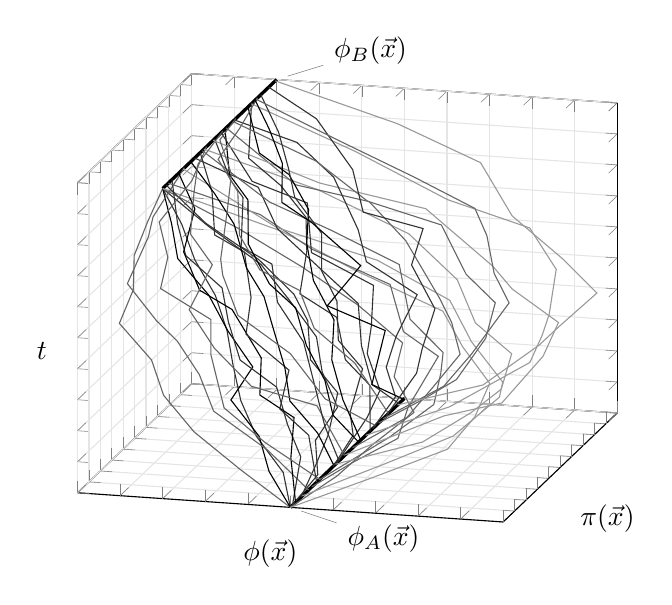
\begin{tikzpicture}
\begin{axis}[
	clip=false,
	view={-75}{20}, 
	%xtick=\empty, ytick=\empty, ztick=\empty, 
	xticklabel=\empty, yticklabel=\empty, zticklabel=\empty,
	xlabel=$\pi(\vec{x})$, ylabel=$\phi(\vec{x})$, zlabel=$t$, zlabel style={rotate=-90},
	%x label style={at={(axis description cs:0.5,0.0)},anchor=north},
	%y label style={at={(axis description cs:0.5,0.0)},anchor=north},
	%z label style={at={(axis description cs:0.5,0.0)},anchor=north},
	xmin=0, xmax=1, ymin=0, ymax=1, zmin=0, zmax=5,
	xtick distance=0.1, ytick distance=0.1, ztick distance=0.5, grid=major, grid style={solid, thin, black!10!white},
	%extra x ticks={0j
	declare function={
		phi1 = 0.5;
		phi2 = 0.8;
		randbetween(\a,\b) = \a + (\b - \a) / 2 * rand;
		%randradius(\x, \rmin, \rmax) = randbetween(\rmin, \rmax) * (\x-0) * (\x-1);
		randfunc(\x,\rmin,\rmax) = randbetween(\rmin,\rmax) * (\x-0)*(\x-1) * 4; % and(x>=0.01, x<=0.99); %(\x-0) * (\x-1);
	},
]
\addplot3 [domain=0:1, samples=2, very thick] ({x}, {phi1}, {0}) node [pos=0.0,pin={-8:$\phi_A(\vec{x})$}] {};
\addplot3 [domain=0:1, samples=2, very thick] ({x}, {phi2}, {5}) node [pos=1.0,pin={+5:$\phi_B(\vec{x})$}] {};
\pgfplotsinvokeforeach{0.0, 0.2, ..., 1.0} {
	\addplot3 [domain=0:1, samples=10, domain y=0:1, samples y=1, black!60!white]  ({max(0, min(1, #1+randbetween(-0.1,0.1))}, {phi1 + (phi2-phi1)*x + randfunc(x,-0.2,-0.3)}, {5*x});
	\addplot3 [domain=0:1, samples=10, domain y=0:1, samples y=1, black!80!white]  ({max(0, min(1, #1+randbetween(-0.1,0.1))}, {phi1 + (phi2-phi1)*x + randfunc(x,-0.0,-0.1)}, {5*x});
	\addplot3 [domain=0:1, samples=10, domain y=0:1, samples y=1, black!100!white] ({max(0, min(1, #1+randbetween(-0.1,0.1))}, {phi1 + (phi2-phi1)*x + randfunc(x,+0.0,+0.1)}, {5*x});
	\addplot3 [domain=0:1, samples=10, domain y=0:1, samples y=1, black!80!white]  ({max(0, min(1, #1+randbetween(-0.1,0.1))}, {phi1 + (phi2-phi1)*x + randfunc(x,+0.2,+0.3)}, {5*x});
	\addplot3 [domain=0:1, samples=10, domain y=0:1, samples y=1, black!60!white]  ({max(0, min(1, #1+randbetween(-0.1,0.1))}, {phi1 + (phi2-phi1)*x + randfunc(x,+0.4,+0.5)}, {5*x});
	\addplot3 [domain=0:1, samples=10, domain y=0:1, samples y=1, black!40!white]  ({max(0, min(1, #1+randbetween(-0.1,0.1))}, {phi1 + (phi2-phi1)*x + randfunc(x,+0.6,+0.7)}, {5*x});
	%\addplot3 [domain=0:1, samples=10, domain y=0:1, samples y=1] ({#1+randfunc(x,0.2,0.3)}, {phi1 + (phi2-phi1)*x + randfunc(x,0.1,0.2)}, {5*x});
}
\end{axis}
\end{tikzpicture}
\caption{\label{fig:phase_space}A quantum system that evolves from the initial field $\phi_A(\vec{x})$ to the final field $\phi_B(\vec{x})$ can take all possible paths through phase space, but some are more likely than others. The conjugate momentum field $\pi(\vec{x})$ does not need to be the same at the start and the end.}
\end{figure}

Substituting \cref{eq:tft:inner_product_position_momentum,eq:tft:path_integral_hamiltonian_assumption,eq:tft:hamiltonian_eigenvalues}, the transition amplitude \eqref{eq:tft:transition_amplitude_product} becomes
\begin{equation}
\begin{split}
	\transampl &=      \left( \prod_{n=1}^N \int \dif \phi_n \int \frac{\dif \pi_n}{2 \pi \hbar} \right) \\
	           &\times \exp \left\{ \frac{i \Delta t}{\hbar} \sum_{n=1}^N \int \dif^3 x \left[ \pi_n(\vec{x}) \frac{\phi_{n+1}(\vec{x}) - \phi_n(\vec{x})}{\Delta t} - \ham \left( \pi_n(\vec{x}), \phi_n(\vec{x}) \right) \right]
	\right\}
\end{split}
\end{equation}
Finally, we take the continuum limit by sending $N \rightarrow \infty$.
It is then natural to define
$\phi(\vec{x}, t_n) = \phi_n(\vec{x}, t_n)$
and
$\pi(\vec{x}, t_n) = \pi_n(\vec{x}, t_n)$
to be the values of the fields at each timestep $t_n$.
Both become continuous functions of time in the continuum limit.
We also use the finite difference definition of the derivative to turn the fraction in the exponential into a partial derivative $\dot{\phi}(\vec{x},t) = \pdv{\phi(\vec{x},t)}/{t}$.
Similarly, we use the Riemann sum definition of the integral to turn the sum $\Delta t\sum$ into an integral $\int \dif t$.
We also define the \textbf{functional integrals}
\begin{equation}
	\int \pathintdif \phi = \lim_{N \rightarrow \infty} \prod_{n=1}^{N} \int \dif \phi_n
	\qquad \text{and} \qquad
	\int \pathintdif \pi = \lim_{N \rightarrow \infty} \prod_{n=1}^{N} \int \frac{\dif \pi_n}{2 \pi \hbar} .
\label{eq:tft:functional_integral}
\end{equation}
%We have swept the diverging factor $(2 \pi \hbar)^N$ under the rug, arguing that it contains no physical information about the dynamics of the process and can be ignored, unlike the other factors.
%TODO: can integrate out momentum with gaussian integral if it appears as $p^2$)
With all of these steps, the transition amplitude takes the form of the \textbf{path integral}
\begin{equation}
\begin{split}
	\transampl &=      \int \pathintdif \pi \int_{\phi(\vec{x}, 0)=\phi_A(\vec{x})}^{\phi(\vec{x},T)=\phi_B(\vec{x})} \pathintdif \phi \\
	           &\times \exp \left\{ \frac{i}{\hbar} \int_0^T \dif t \int \dif^3 x \left[ \pi(\vec{x}, t) \dot{\phi}(\vec{x}, t) - \ham \left( \pi(\vec{x}, t), \phi(\vec{x}, t) \right) \right] \right\} .
\end{split}
\label{eq:tft:path_integral_hamiltonian}
\end{equation}

It is tempting to recognize $\pi \dot\phi - \ham$ as the Legendre transformation that converts to the Lagrangian density and write $\lagr$ in its place.
But we should be careful -- the Legendre transformation converts the independent variable $\dot\phi$ in $\lagr(\phi, \dot\phi, \nabla\phi)$ to $\pi$ in $\ham(\phi, \pi, \nabla\phi)$.
We are integrating over $\pi$ and should therefore not lose track of it by writing $\lagr = \lagr(\phi, \dot\phi, \nabla\phi)$.
Thus, we do not modify the integral further.
\TODO{does this make sense?}

\iffalse
Note that the combination of the Hamiltonian and the fields in the exponential is precisely the Legendre transformation that converts between the Hamiltonian density $\ham$ and the Lagrangian density $\lagr$.
Thus, we might as well express the transition amplitude as the \textbf{path integral}
%	\transampl = \int \pathintdif \pi \int_{\phi_A(\vec{x}, 0)}^{\phi_B(\vec{x}, T)} \pathintdif \phi \\
%	             \exp \left( i \int_0^T \dif t \int \dif^3 x \, \left( \lagr(\pi(\vec{x}, t), \phi(\vec{x}, t)) \right) \right) .
\begin{equation}
	\transampl = \int \pathintdif \pi \int_{\phi_A(\vec{x})}^{\phi_B(\vec{x})} \pathintdif \phi \, \exp \big( i S \left[ \pi(\vec{x}, t), \phi(\vec{x}, t) \right] / \hbar \big) ,
\label{eq:tft:path_integral_lagrangian}
\end{equation}
with the action
\begin{equation}
	S \left[ \pi(\vec{x}, t), \phi(\vec{x}, t) \right] = \int_0^T \dif t \int \dif^3 x \, \lagr \left( \pi(\vec{x}, t), \phi(\vec{x}, t) \right) . \qquad \text{TODO: factor $c$?}
\label{eq:tft:action}
\end{equation}
\fi
The path integral expresses the transition amplitude for the process $A \rightarrow B$ as a sum over all possible paths through phase space, each weighted by the value on the unit circle with phase corresponding to the action of the path.
This interpretation is illustrated in \cref{fig:phase_space}.
Note that the position-space integral $\int \pathintdif \phi$ is constrained to start and end in the initial and final states due to the leftmost and righmost products with $\bra{\phi_B}$ and $\ket{\phi_A}$, but the momentum integral $\int \pathintdif \pi$ has no such constraint.

Why have we spent so much time on this transition amplitude, when we really are only interested in the partition function \eqref{eq:tft:partition_function}?
If we evaluate the trace \eqref{eq:tft:partition_function} in the basis of fields $\ket{\phi_0}$, we obtain
\begin{equation}
	Z = \int \dif \phi_0 \Braket{\phi_0 | e^{-\beta (\hat{H} - \mu_i \hat{N}_i)} | \phi_0} .
\end{equation}
This is precisely an integral over transition amplitudes \eqref{eq:tft:path_integral_hamiltonian}, but now with 
\begin{itemize}
\item equal start and end states $\ket{\phi_A} = \ket{\phi_B} = \ket{\phi_0}$, 
\item the Hamiltonian $\hat{H} - \mu_i \hat{N}_i$ and 
\item a purely imaginary time variable $t = -i \tau$ with $\tau$ running from $0$ to $\beta \hbar$.
\end{itemize}
Thus, we can express the partition function as path integrals \eqref{eq:tft:path_integral_hamiltonian} with these simple substitutions!
We redefine the field $\phi(\vec{x}, t) \rightarrow \phi(\vec{x}, \tau)$ to be functions of the new ``time'' $\tau$.
Therefore, we substitute $i \int \dif t \rightarrow \int \dif \tau$ and $\dot\phi(x, t) = \pdv{\phi(\vec{x},t)}/{t} \rightarrow \pdv{\phi(\vec{x},\tau)}/{(-i \tau)} = i \dot\phi(\vec{x},\tau)$.
Omitting the arguments of the fields from now, we obtain
\begin{equation}
	Z = \int \pathintdif \pi \oint_+ \pathintdif \phi \, \exp \left[ \frac{1}{\hbar} \int_0^{\beta \hbar} \dif \tau \int \dif^3 x \left( i \pi \dot{\phi} - \ham + \mu \numdensity \right) \right]
\label{eq:tft:bosonic_partition_function}
\end{equation}
where we have absorbed $\int \dif \phi_0$ into the path integral $\int \pathintdif \phi$ and write $\oint_+$ to indicate that we integrate over all fields $\phi(x, \tau) = \phi(x, \tau + \beta \hbar)$ that are \emph{periodic} in $\tau$, due to the equal start and end states $\phi_A(\vec{x}) = \phi_B(\vec{x})$ in \cref{eq:tft:path_integral_hamiltonian}.
Thus, thermal field theory -- statistical mechanics for quantum fields at finite temperature -- is essentially equivalent to ordinary quantum field theory with temperature-dependent time and periodic fields, and the partition function is obtained by integrating along closed paths in phase space!

We have not yet discussed the appearance of the chemical potential $\mu$ and the number density $\numdensity$ in the path integral.
If the theory admits one or more conserved conserved currents $j_i^\mu$ with $\partial_\mu j_i^\mu$ by Noether's theorem, there are associated conserved charges $Q_i = \int \dif^3 x \, j_i^0$.
For every such conserved charge, we can associate a chemical potential $\mu_i$ and include the term
\begin{equation}
	\mu_i \numdensity_i = \mu_i j_i^0
\label{eq:tft:chemical_potential}
\end{equation}
in the path integral.
For example, if the theory has particles and antiparticles, then a conserved charge typically corresponds to the difference between the number of particles and antiparticles in the system.
The chemical potential can then be interpreted as a knob with which we can regulate the balance between particles and antiparticles in the system.
We will later see examples of theories both with and without conserved charges.

\TODO{i do not understand properly how the chemical potential works and why we can include it}

\section{Path integral for fermionic partition function}

%\newcommand\creat[1]{\hat\psi^\dagger(\vec{#1})}
%\newcommand\destr[1]{\hat\psi        (\vec{#1})}
\newcommand\creat{\hat\psi^\dagger}
\newcommand\destr{\hat\psi        }

We will now develop a path integral for a fermionic field $\psi(\vec{x})$.
For example, the Dirac Lagrangian is $\lagr = \bar{\psi} (i \hbar c \slashed\partial - m c^2) \psi$ with conjugate momentum $\pi = \fdv{\lagr}/{\dot\psi} = i \hbar \psi^\dagger$, so we are instructed to treat the field and its conjugate independently in the path integral.
This is not a peculiarity of fermionic fields only -- for a complex scalar field $\phi$, for example, we would also be instructed to treat $\phi$ and $\conj\phi$ separately. 

Why do we need to derive the path integral for fermions separately -- can we not just use the bosonic path integral \eqref{eq:tft:bosonic_partition_function} with the appropriate conjugate momentum?
By assumption, the fermion field operator $\destr(\vec{x})$ and its conjugate $\creat(\vec{x})$ obey the fermionic \textbf{anticommutation relations}
\begin{equation}
\begin{split}
	\acomm{\destr(\vec{x})}{\creat(\vec{y})} = \acomm{\creat(\vec{y})}{\destr(\vec{x})} &= \delta(\vec{x}-\vec{y}) , \\
	\acomm{\creat(\vec{x})}{\creat(\vec{y})} = \acomm{\destr(\vec{x})}{\destr(\vec{y})} &= 0 ,
\end{split}
\label{eq:tft:fermion_anticommutators}
\end{equation}
in contrast to the bosonic commutators \eqref{eq:tft:boson_field_commutators}.
In the derivation of the bosonic path integral \eqref{eq:tft:bosonic_partition_function}, we treated the eigenvalues $\phi$ and $\pi$ of the operators $\hat\phi$ and $\hat\pi$ as ordinary numbers.
However, the anticommutators \eqref{eq:tft:fermion_anticommutators} of the fermionic field operators in fact requires their eigenvalues to anticommute!
For example,
\begin{equation}
\begin{split}
	\text{if}   \quad & \destr \ket{\psi} = \psi \ket{\psi} , \\
	\text{then} \quad & \braket{\psi | \creat \destr | \psi} = \braket{\psi | \conj\psi \psi | \psi} = -\braket{\psi | \psi \conj\psi | \psi} = -\braket{\psi | \destr \creat | \psi} \quad \text{by \eqref{eq:tft:fermion_anticommutators}}, \\
	\text{so}   \quad & \acomm{\psi}{\conj\psi} = 0 . \\
\end{split}
\label{eq:tft:eigenvalues_must_anticommute}
\end{equation}
By similar reasoning, one can also deduce the requirements $\acomm{\psi}{\creat} = \acomm{\psi}{\destr} = 0$.
The bosonic path integral \eqref{eq:tft:bosonic_partition_function} and its derivation is therefore not valid for fermions.

To develop the fermionic path integral, we therefore replace the algebra of ordinary commuting numbers in the bosonic case with anticommuting \textbf{Grassmann numbers}.
Assuming most readers have encountered them before, we define and derive all properties of Grassmann numbers that will be useful to us in \cref{chap:grassmann_numbers} and will only refer to them in this section.
\TODO{big A in Appendix etc?}

In the derivation of the bosonic path integral \eqref{eq:tft:bosonic_partition_function}, we relied heavily on using eigenstates of the system to take the trace in \eqref{eq:tft:partition_function}, insert completeness relations and take inner products between eigenstates.
To find analogous ways of doing this with fermionic fields, we will introduce \textbf{fermionic coherent states}.

\iffalse
To compute the fermionic path integral, we must therefore replace the algebra of commuting complex numbers in the bosonic case with the algebra of anticommuting \textbf{Grassmann numbers}.
This algebra was invented by the German mathematician Hermann Grassmann in the 19th century.
His work did not gain much traction at that time.
In fact, the publisher of one of his book once wrote to him that
\emph{``(...) since your work hardly sold at all, roughly 600 copies were used in 1864 as waste paper and the remaining few odd copies have now been sold out, with the exception of the one copy in our library.''}
Grassmann was so disappointed with the reception of his work that he turned to study linguistics the last years of his life.
Today, however, his work on Grassmann numbers is the whole fundament for the construction of the fermionic path integral, and his other work is also very important \TODO{fix}.
We review Grassmann numbers in \TODO{ref appendix}.

For concreteness, consider fermions described by the Dirac Lagrangian
\begin{equation}
	\lagr = \bar{\psi} (i \hbar c \slashed\partial - m c^2) \psi .
\end{equation}
Here, the conjugate momentum turns out to be
\begin{equation}
	\pi = \fdv{\lagr}{\dot\psi} = i \hbar \psi^\dagger ,
\label{eq:tft:dirac_conjugate_momentum}
\end{equation}
so, perhaps confusingly, we are instructed to treat the field and its conjugate as independent variables in the path integral.
\fi

Let us get to work.
Suppose we have a finite number $N$ of Grassmann numbers $\psi_i$ and equally many creation and destruction \TODO{annihiliation?} operators $\creat_i$ and $\destr_i$.
Following the discussion around \cref{eq:tft:eigenvalues_must_anticommute} \TODO{vague} and the definition of Grassmann numbers in \cref{chap:grassmann_numbers}, we have, by assumption, all the anticommutators
\begin{equation}
\begin{split}
	\acomm{\psi_i}{\psi_j} = \acomm{\psi_i}{\conj\psi_j} = \acomm{\conj\psi_i}{\conj\psi_j}                             &= 0            , \\
	\acomm{\psi_i}{\destr_j} = \acomm{\psi_i}{\creat_j} = \acomm{\conj\psi_i}{\destr_j} = \acomm{\conj\psi_i}{\creat_j} &= 0            , \\
	\acomm{\destr_i}{\destr_j} = \acomm{\creat_i}{\creat_j}                                                             &= 0            , \\
	\acomm{\destr_i}{\creat_j} = \acomm{\creat_j}{\destr_i}                                                             &= \delta_{i j} . \\
\end{split}
\label{eq:tft:fermionic_all_anticommutators}
\end{equation}
In other words, all field operators and all Grassmann numbers anticommute with themselves and each other.
The anticommutators \eqref{eq:tft:fermionic_all_anticommutators} of the field operators $\creat_i$ and $\destr_i$ are the discrete analogues of \eqref{eq:tft:fermion_anticommutators}.
It will be less painful \TODO{brutal?} to describe the formalism of fermionic coherent states in the discrete case and then take the continuum limit $\psi_i \rightarrow \psi(\vec{x})$ in the end.

The Fock space of the fermionic field has a \textbf{ground state} or \textbf{vacuum state} that we denote by
\begin{equation}
	\ket{0, 0, \ldots, 0} = \ket{0}. \\
\end{equation}
We can apply any sequence of $n = \sum_i n_i$ different creation operators to it to build an \textbf{$n$-particle state}
\begin{equation}
	\ket{n_1, n_2, \ldots, n_N} = \left( \creat_1 \right)^{n_1} \cdots \left( \creat_N \right)^{n_N} \ket{0} .
\label{eq:tft:fermionic_many_particle_state}
\end{equation}
This results in a non-zero state only if $n_i \in \{0, 1\}$ for all $i$, because $(\creat_i)^2 \ket{0} = -(\creat_i)^2 \ket{0} = 0$ by the anticommutator \eqref{eq:tft:fermionic_all_anticommutators}.
Note that shuffling the sequence of operators in \cref{eq:tft:fermionic_many_particle_state} can change the sign -- we define the $n$-particle state to have operators with indices that increase from left to right.
In particular, we can build the \textbf{one-particle state}
\begin{equation}
	\ket{1_i} = \ket{(n_1=0), \ldots, (n_i=1), \ldots, (n_N=0)} = \creat_i \ket{0} .
\end{equation}
Note also that $\creat_i \ket{1_i} = (\creat_i)^2 \ket{0} = -(\creat_i)^2 \ket{0} = 0$.
Therefore we have
\begin{equation}
	\destr_i \ket{1_i} = \destr_i \creat_i \ket{0} = (1 - \creat_i \destr_i) \ket{0} = \ket{0} .
\end{equation}
The interpretation of this analysis is that the \textbf{creation operator} $\creat_i$ adds a particle in the state $i$, while the \textbf{destruction operators} $\destr_i$ removes a particle from the same state.
The restriction that $n_i \in \{0, 1\}$ implies that there can be at most one particle in every state, consistent with the Pauli exclusion principle.
Note that the Fock space has a total of $2^N$ distinct states
\begin{equation}
	\ket{n_1, n_2, \ldots, n_N} \qquad \text{where } n_i \in \{0, 1\} \text{ for all } i = 1, \ldots, N .
\label{eq:tft:fermion_all_states}
\end{equation}

Next, define the \textbf{coherent state}
\begin{equation}
	\ket{\psi} = \exp \left( -\sum_i \psi_i \creat_i \right) \ket{0} = \prod_i \exp \left( -\psi_i \creat_i \right) \ket{0} = \prod_i \left( 1 - \psi_i \creat_i \right) \ket{0} .
\end{equation}
In the last line, we made use of the Taylor expansion \eqref{eq:gnums:function_taylor_series} of functions of Grassmann numbers.
Applying a destruction operator to this state gives
\begin{equation}
\begin{aligned}
	%\destr_j \ket{\psi} = \psi_j \ket{0} = \psi_j \ket{\psi} \quad \text{(last because $\psi_j^2=0$)}
	%\destr_j \ket{\psi} = \destr_j \prod_i \left( 1 - \psi_i \creat_i \right) \ket{0} = + \psi_j \destr_j \creat_j \ket{0} = \psi_j \ket{0} .
	\destr_j \ket{\psi} &= \destr_j \prod_i \left( 1 - \psi_i \creat_i \right) \ket{0} = \prod_{i \neq j} \left( 1 - \psi_i \creat_i \right) \destr_j \left( 1 - \psi_j \creat_j \right) \ket{0} \\
	                    &= \prod_{i \neq j} \left( 1 - \psi_i \creat_i \right) \psi_j \ket{0} = \prod_{i \neq j} \left( 1 - \psi_i \creat_i \right) \psi_j \left( 1 - \psi_j \creat_j \right) \ket{0}   \\
	                    &= \psi_j \prod_i \left( 1 - \psi_i \creat_i \right) \ket{0} = \psi_j \ket{\psi} . \\
\end{aligned}
\end{equation}
In other words, the coherent state $\ket{\psi}$ is an eigenstate of every destruction operator $\destr_j$ with eigenvalue $\psi_j$!
This is analogous to the bosonic eigenequation \TODO{eigen equation?} \eqref{eq:tft:field_eigenvalue_equations}.
It is the coherent states that we wish to use when taking the trace, inner product and inserting identity operators in the path integral.

First, let us find the inner product between two coherent states.
It is
\begin{equation}
\begin{split}
	\iffalse
	\braket{\psi | \psi'} &= \braket{0 | \prod_i (1 - \destr_i \conj\psi_i) \prod_j (1 - \psi'_j \creat_j) | 0} \\
	                      &= \braket{0 | 0} + \sum_{i,j} \braket{0 | \destr_i \conj\psi_i \psi'_j \creat_j | 0}
	                       = \braket{0 | 0} + \sum_{i,j} \conj\psi_i \psi'_j \braket{0 | \destr_i \creat_j | 0} \\
	                      &= \braket{0 | 0} + \sum_{i  } \conj\psi_i \psi'_i
						   = 1 + \sum_i \conj\psi_i \psi'_i = \exp \left( \sum_i \conj\psi_i \psi'_i \right) .
	\fi
	\Braket{\psi | \psi'} &= \Braket{\psi | \prod_i (1 - \psi'_i \creat_i) | 0} = \Braket{\psi | \prod_i (1 + \creat_i \psi'_i) | 0} = \Braket{\psi | \prod_i (1 + \conj\psi_i \psi'_i) | 0} \\
						  &= \underbrace{\Braket{0 | 0}}_{1} \prod_i (1 + \conj\psi_i \psi'_i) = \prod_i \exp(\conj\psi_i \psi'_i) = \exp \left( \sum_i \conj\psi_i \psi'_i \right) .
\end{split}
\label{eq:tft:grassmann_inner_product_discrete}
\end{equation}

Next, we can work out that the unit operator $\hat{1}$ \TODO{use cool font} can be represented by the integral
\begin{equation}
\begin{split}
	 \iffalse
	 & \int \dif \conj{\psi} \int \dif \psi \, e^{-\sum_i \conj\psi_i \psi_i} \ket{\psi} \bra{\psi} \\
	=& \int \dif \conj{\psi} \int \dif \psi \, \prod_i \left( 1 + \psi_i \conj{\psi}_i \right) \prod_j \left( 1 - \psi_j \creat_j \right) \ket{0} \bra{0} \prod_k \left( 1 - \destr_k \conj\psi_k \right) \\
	=& \int \dif \conj{\psi} \int \dif \psi \, \prod_i \left( 1 + \psi_i \conj{\psi}_i \right) \prod_j \left( 1 - \psi_j \creat_j \right) \ket{0} \bra{0} \left( 1 - \destr_j \conj\psi_j \right) \\
	=& \sum_{n_1=0}^1 \sum_{n_2=0}^1\cdots \sum_{n_N=0}^1 \ket{n_1, n_2, \ldots, n_N} \bra{n_1, n_2, \ldots, n_N} = \hat{1} \\
	=& \int \dif \conj{\psi} \int \dif \psi \left[ \left( -\sum_i \conj{\psi}_i \psi_i \right) \ket{0} \bra{0} + \left( -\sum_j \psi_j \creat_j \right) \ket{0} \bra{0} \left( -\sum_k \destr_k \conj\psi_k \right) \right] \\
	=& \int \dif \conj{\psi} \int \dif \psi \left[ \sum_i \psi_i \conj\psi_i \ket{0} \bra{0} + \sum_{j,k} \psi_j \conj\psi_k \ket{1_j} \bra{1_k} \right] \\
	=& \ket{0} \bra{0} + \sum_j \ket{1_j} \bra{1_j} = \hat{1} . \\
	\fi
	 & \int \dif \conj{\psi} \int \dif \psi \, \exp \left( -\sum_i \conj\psi_i \psi_i \right) \ket{\psi} \bra{\psi} \\
	=& \int \dif \conj{\psi} \int \dif \psi \, \prod_i \left( 1 + \psi_i \conj{\psi}_i \right) \prod_j \left( 1 - \psi_j \creat_j \right) \ket{0} \bra{0} \prod_k \left( 1 - \destr_k \conj\psi_k \right) \\
	=& \sum_{n_1=0}^1 \sum_{n_2=0}^1\cdots \sum_{n_N=0}^1 \ket{n_1, n_2, \ldots, n_N} \bra{n_1, n_2, \ldots, n_N} = \hat{1} . \\
\end{split}
\label{eq:tft:completeness_grassmann_discrete}
\end{equation}
To make the big leap across the second equality sign, stare intensely at the middle \TODO{penaltimate ????} line while following the next argument.
To get a non-zero contribution from the integral, the parentheses must be multiplied out in a way such that one gets terms with the particular combination
\begin{equation}
	\int \dif \conj\psi \int \dif \psi \, \psi_1 \conj\psi_1 \cdots \psi_N \conj\psi_N = 1 .
\label{eq:tft:integral_saturated}
\end{equation}
Any term with duplicate fields $\psi_i^2 = -\psi_i^2 = 0$ will yield zero, and so will terms with products that do not include \emph{all} $\psi_i$ and $\conj\psi_i$ due to the integration properties \eqref{eq:gnums:integration_differentiation} and the discussion surrounding \cref{eq:gnums:integration_over_all} \TODO{vague}.
Based on this, we can derive three rules for what combinations of factors we can choose when multiplying out the three parentheses. \TODO{product?}
\begin{enumerate}
\item \textbf{For any $i$ in the first parenthesis:} Given that we follow the two next rules, we are free to choose either the factor $1$ or $\psi_i \conj\psi_i$. \label{eq:tft:logic_tree_one}
\item \textbf{For $j=i$ in the second parenthesis:} 
If we choose $\psi_i \conj\psi_i$ in the first parenthesis, we \emph{must} choose $1$ in the second to avoid a duplicate factor $\psi_i^2 = 0$.
Conversely, if we choose $1$ in the first, we \emph{must} choose $-\psi_j \creat_j$ in the second to ``saturate'' the field product.
\item \textbf{For $k = j = i$ in the third parenthesis:} 
If we choose $-\psi_j \creat_j$ in the second, we \emph{must} choose $-\psi_k \creat_k$ in the third to get $\psi_j \conj\psi_j$ in the field product.
Conversely, if we choose $1$ in the second, then we have already included $\psi_i \conj\psi_i$ from rule \ref{eq:tft:logic_tree_one}, and we \emph{must} choose $1$ in the third to not ``oversaturate'' the field product. \label{eq:tft:logic_tree_three}
\end{enumerate}
Following these rules, the first parenthesis expands to all possible $2^N$ terms.
For every one of these terms, there is precisely one legal \TODO{different word, it is ``legal''..} combination of factors to choose in the second and third parentheses.
This evaluates to $2^N$ terms with all possible combinations of $N_j = N_k$ creation and annihilation operators and $N_i = N - N_j$ Grassmann numbers.
\emph{These $2^N$ terms are therefore precisely all the $2^N$ states \eqref{eq:tft:fermion_all_states} in the Fock space!}
The sign ambiguity following different orders of operators in the state \eqref{eq:tft:fermionic_many_particle_state} does not cause any problems with signs in the sum over all the states, either.
To understand why, note that rule \ref{eq:tft:logic_tree_three} forces us to apply the same sequence of operators to both $\ket{0}$ and $\bra{0}$, and any ordering that does not follow definition \eqref{eq:tft:fermionic_many_particle_state} can be made to do so, because anticommuting the same operators in each sequence would introduce \emph{two} negative signs that cancel.
This explains the transition to the final line.
\iffalse
\begin{itemize}
\item choose $k = j$ in the third parenthesis in order to pair $\psi_j$ with $\conj\psi_j$, and
\item for every factor $\psi_i \conj\psi_i$ one chooses from the first parenthesis, one must choose the factor $1$ from the second and third parentheses in order to avoid $\psi_i^2=0$, and conversely,
\item for every factor $1$ one chooses from the first parenthesis, one must choose the factor $-\psi_j \creat_j$ and $-\destr_k \conj\psi_k$ from the second and third parentheses in order to not miss a factor $\psi_i \conj\psi_i$ in the product \TODO{ref}.
\end{itemize}
Following these rules is equivalent to iterating over all $2^N$ combinations with $N_j$ creation and destruction operators in the second and third parentheses and $N_i = N - N_j$ Grassmann numbers in the first parenthesis.
\fi
To be clear, the very last equality follows because the sum goes over all states \eqref{eq:tft:fermion_all_states} in the Fock space.

With the same reasoning, we can work out that the trace of an operator $\hat{A}$ can be written
\begin{equation}
\begin{split}
	 & \int \dif \conj{\psi} \int \dif \psi \, \exp \left( -\sum_i \conj{\psi}_i \psi_i \right) \Braket{-\psi | \hat{A} | \psi} \\
	=& \int \dif \conj{\psi} \int \dif \psi \, \prod_i (1 + \conj\psi_i \psi_i) \Braket{0 | \prod_j (1 + \destr_j \conj\psi_j) \hat{A} \prod_k (1 - \psi_k \creat_k) | 0} \\
	=& \int \dif \conj{\psi} \int \dif \psi \, \prod_i (1 + \conj\psi_i \psi_i) \Braket{0 | \prod_j (1 + \destr_j \conj\psi_j) \hat{A} (1 - \psi_j \creat_j) | 0} \\
	%=& \int \dif \conj{\psi} \int \dif \psi \, \prod_i (1 + \conj\psi_i \psi_i) \prod_j \conj\psi_j \psi_j \Braket{0 | (1 + \destr_j \psi_j) \hat{A} (1 + \conj\psi_j \creat_j) | 0} \\
	=& \sum_{n_1=0}^1 \sum_{n_2=0}^1\cdots \sum_{n_N=0}^1 \Braket{n_1, n_2, \ldots, n_N | \hat{A} | n_1, n_2, \ldots, n_N} = \trace{\hat{A}} . \\
	%=& \int \dif \conj{\psi} \int \dif \psi \left[ (-\sum_i \conj\psi_i \psi_i) \Braket{0 | \hat{A} | 0} + \Braket{0 | (+\sum_j \destr_j \conj\psi_j) \hat{A} (-\sum_k \psi_k \creat_k) | 0} \right] \\
	%=& \int \dif \conj{\psi} \int \dif \psi \left[ \sum_i \psi_i \conj\psi_i \Braket{0 | \hat{A} | 0} + \sum_{j,k} \psi_k \conj\psi_j \Braket{1_j | \hat{A} | 1_k} \right] \\
	%=& \Braket{0 | \hat{A} | 0} + \sum_j \Braket{1_j | \hat{A} | 1_j} = \trace{\hat{A}} . \\
\end{split}
\label{eq:tft:trace_grassmann_discrete}
\end{equation}
Across the third equality, we (anti)commute $\psi_j$ and $\conj\psi_j$ all the way to the left to write $\braket{0 | \destr_j \conj\psi_j \hat{A} (-\psi_j \creat_j) | 0} = \psi_j \conj\psi_j \braket{0 | \destr_j \hat{A} \creat_j | 0}$ while assuming that $\hat{A}$ is a ``bosonic'' operator that \emph{commutes} with the Grassmann numbers.
The Hamiltonian \eqref{eq:tft:dirac_hamiltonian} for a Dirac field that we encounter later is one example of such an $\hat{A}$, as it contains two field operators.

\TODO{dirac field should have indices in its anticommutation relations}

As we remarked at the start, this analysis was for discrete fields that satisfy the discrete anticommutators \eqref{eq:tft:fermionic_all_anticommutators}.
We are studying fields $\psi(\vec{x})$ and $\conj\psi(\vec{x})$ with an infinite number of field operators $\creat(\vec{x})$ and $\destr(\vec{x})$ that satisfy the continuum generalization \eqref{eq:tft:fermion_anticommutators}.
Our results carry over with the substitutions $\psi_i \rightarrow \psi(\vec{x})$, as if every Grassmann number corresponds to the field at one position, and $\sum_i \rightarrow \int \dif^3 x$.
For example, we would rather define the coherent state
\TODO{remove hypothetical tense}
\begin{equation}
	\ket{\psi} = \exp \left[ -\int \dif^3 x\, \psi(\vec{x}) \hat\psi^\dagger(\vec{x}) \right] \ket{0} .
\end{equation}
The inner product \eqref{eq:tft:grassmann_inner_product_discrete} between two coherent states would then become
\begin{equation}
	\braket{\psi | \psi'} = \exp \left[ \int \dif^3 x \, \conj\psi(\vec{x}) \psi'(\vec{x}) \right]
\label{eq:tft:grassmann_inner_product}
\end{equation}
The identity operator \eqref{eq:tft:grassmann_inner_product_discrete} would then become
\begin{equation}
	\int \dif \conj\psi \int \dif \psi \, \exp \left[ -\int \dif^3 x \, \conj\psi(\vec{x}) \psi(\vec{x}) \right] \ket{\psi} \bra{\psi} = \hat{1} ,
\label{eq:tft:completeness_grassmann}
\end{equation}
\TODO{cool font for 1}
while the trace \eqref{eq:tft:trace_grassmann_discrete} would turn out to be
\begin{equation}
	\int \dif \conj\psi \int \dif \psi \, \exp \left[ -\int \dif^3 x \, \conj\psi(\vec{x}) \psi(\vec{x}) \right] \Braket{-\psi | \hat{A} | \psi} = \trace{A} .
\label{eq:tft:trace_grassmann}
\end{equation}
The most important thing to note is the negative sign in $\bra{-\psi}$ of the trace \eqref{eq:tft:trace_grassmann} -- we will see that this requires fermionic fields to be \emph{antiperiodic} in imaginary time, in contrast to the periodic bosonic fields.

Let us now build \TODO{build?} the path integral for the fermionic partition function using \cref{eq:tft:grassmann_inner_product,eq:tft:completeness_grassmann,eq:tft:trace_grassmann} as our toolbox. \TODO{... FROM our toolbox eq 123 ...?}
The partition function \eqref{eq:tft:partition_function} follows from the trace \eqref{eq:tft:trace_grassmann} with $\hat{A} = e^{-\beta (\hat{H} - \mu \hat{N})}$ as
\begin{equation}
	Z = \int \dif \psi_0^\dagger \int \dif \psi_0 \, e^{-\int \dif^3 x \, \psi_{0}^\dagger(\vec{x}) \psi_{0}(\vec{x})} \Braket{-\psi_0 | e^{-\beta(\hat{H} - \mu \hat{N})} | \psi_0} .
\label{eq:tft:fermion_path_integral_after_completeness}
\end{equation}
Breaking up the operator $e^{-\beta (\hat{H} - \mu \hat{N})}$ as in \cref{eq:tft:time_evolution_splitting} with small times $\Delta \tau = \beta \hbar / N$ and inserting one Grassmann completeness relation \eqref{eq:tft:completeness_grassmann} between every factor, the partition function becomes
\begin{equation}
	Z = \prod_n \int \dif \psi_n^\dagger \int \dif \psi_n \, e^{-\int \dif^3 x \, \psi_{n+1}^\dagger(\vec{x}) \psi_{n+1}(\vec{x})} \Braket{\psi_{n+1} | e^{-(\hat{H} - \mu \hat{N}) \Delta \tau / \hbar} | \psi_n} ,
\end{equation}
where we define $\bra{\psi_{N+1}} = \bra{-\psi_0}$ -- \emph{note the minus sign!}
Next, expand the Hamiltonian to first order as in \cref{eq:tft:path_integral_hamiltonian_assumption}.
Then we obtain
\begin{equation}
	Z = \prod_n \int \dif \psi_n^\dagger \int \dif \psi_n \, e^{-\int \dif^3 x \, \psi_{n+1}^\dagger(\vec{x}) \psi_{n+1}(\vec{x})} \braket{\psi_{n+1} | \psi_n} e^{-(H_n - \mu N) \Delta \tau / \hbar} .
\end{equation}
Now use the Grassmann inner product \eqref{eq:tft:grassmann_inner_product} to write
\begin{equation}
	Z = \prod_n \int \dif \psi_n^\dagger \int \dif \psi_n \, \exp \left[ \frac{\Delta \tau}{\hbar} \sum_n \int \dif^3 x \left( -\hbar \psi^\dagger_{n+1} \frac{\psi_{n+1} - \psi_n}{\Delta \tau} \psi_{n} - \ham + \mu \numdensity \right) \right] .
\end{equation}
% integrate by parts? %why is this valid for Grassmann numbers? Can one e.g. show that $\pdv{\phi^\dagger \phi}{\tau} = 0$?, change order/use int by parts correctly % TODO: don't need this, should rather be careful about index placement above (especially the exp(.. n+1 ..) from completeness)
Finally, take the continuum limit and introduce the functional integrals $\pathintdif \psi = \lim_{N \rightarrow \infty} \prod_n \dif \psi_n$ and $\pathintdif [i \hbar \psi^\dagger] = \lim_{N \rightarrow \infty} \prod_n \dif \psi^\dagger$, where we absorb some physically irrelevant prefactors into the latter to preserve similarity between the conjugate momentum $\pi$ and $i \hbar \psi^\dagger$. 
We then obtain the \textbf{fermionic partition function}
\begin{equation}
	Z = \oint_- \pathintdif [i \hbar \psi^\dagger] \oint_- \pathintdif \psi \exp \left[ \frac{1}{\hbar} \int_0^{\beta \hbar} \dif \tau \int \dif^3 x \left( -\hbar \psi^\dagger \dot{\psi} - \ham \left( \psi^\dagger, \psi \right) + \mu \numdensity \right) \right] ,
\label{eq:tft:fermion_partition_function}
\end{equation}
where $\oint_-$ means to integrate over \emph{antiperiodic} fields $\psi(\vec{x}, 0) = -\psi(\vec{x}, \beta \hbar)$, naturally extending the symbol $\oint_+$ we introduced for bosonic fields that were \emph{periodic}.
Here, antiperiodicity follows from the negative sign in $\bra{-\psi}$ in \cref{eq:tft:trace_grassmann} that we hid in $\bra{\psi_{N+1}} = \bra{-\psi_0}$ right after \cref{eq:tft:fermion_path_integral_after_completeness}.
Remarkably, this result looks identical to the bosonic partition function \eqref{eq:tft:bosonic_partition_function} with canonical momentum $\pi = i \hbar \psi^\dagger$, but here we integrate over Grassmann fields that are antiperiodic.

\iffalse
The partition function is therefore
\begin{equation}
\begin{split}
	Z &= \int \dif \psi_0^\dagger \int \dif \psi_0 \, e^{-\psi_{n+1}^\dagger \psi_{n+1}} \braket{-\psi_0 | e^{-\beta(\hat{H} - \mu \hat{N})} | \psi_0} \\
	  &= \prod_n \int \dif \psi_n^\dagger \int \dif \psi_n \, e^{-\psi_{n+1}^\dagger \psi_{n+1}} \braket{\psi_{n+1} | e^{-(\hat{H} - \mu \hat{N}) \Delta \tau / \hbar} | \psi_n} \\
	  &= \prod_n \int \dif \psi_n^\dagger \int \dif \psi_n \, e^{-\psi_{n+1}^\dagger \psi_{n+1}} \braket{\psi_{n+1} | \psi_n} e^{-(H_n - \mu N) \Delta \tau / \hbar} \\
	  &= \prod_n \int \dif \psi_n^\dagger \int \dif \psi_n \, \exp \left\{ -\frac{\Delta t}{\hbar} \sum_n \int \dif^3 x \left( \psi^\dagger_{n+1} \frac{\psi_{n+1} - \psi_n}{\Delta t} + \ham - \mu \numdensity \right) \right\} \\
	  &= \oint_- \pathintdif \psi^\dagger \oint_- \pathintdif \psi \exp \left\{ \frac{1}{\hbar} \int_0^{\beta \hbar} \dif \tau \int \dif^3 x \left( -\psi^\dagger(\vec{x},\tau) \dot{\psi}(\vec{x},\tau) - \ham \left( \psi^\dagger(\vec{x},\tau), \psi(\vec{x},\tau) \right) + \mu \numdensity \right) \right\} \\
\end{split}
\end{equation}
\fi

\section{Matsubara frequencies}

We have just seen how the partition function for bosons can be expressed by the path integral \eqref{eq:tft:bosonic_partition_function} with fields that are periodic in imaginary time.
For Dirac fermions, we have showed that we can ``naively'' use the same result by substituting the canonical momentum $\pi = i \hbar \psi^\dagger$ and integrate over antiperiodic fields.
In summary, the field $\psi(\vec{x}, \tau)$ -- here regarded as \emph{either} a bosonic or fermionic field -- satisfies the (anti)periodicity
\begin{equation}
	\phi(\vec{x}, \tau) = \begin{cases}
						      + \phi(\vec{x}, \tau + \beta \hbar) & \text{for bosons} \\
						      - \phi(\vec{x}, \tau + \beta \hbar) & \text{for fermions} .
	                      \end{cases}
\label{eq:tft:periodicity}
\end{equation}
Accordingly, we can expand either field in a Fourier series
\begin{equation}
	\psi(\vec{x}, \tau) = \sum_n \psi_n(\vec{x}) e^{i \omega_n \tau}
\end{equation}
with \textbf{Matsubara frequencies} 
\begin{equation}
	\omega_n = \begin{cases}
			       2 \pi n / \beta \hbar    & \text{for bosons} \\
				   2 \pi (n+\frac12) / \beta \hbar & \text{for fermions} .
	           \end{cases}
\label{eq:tft:matsubara_frequencies}
\end{equation}
The offset $+\pi / \beta \hbar$ makes the fermionic field antiperiodic at $\tau = \beta \hbar$.

Although the field is not periodic in space, we can still represent it by its Fourier transform as
\begin{equation}
	\psi_n(\vec{x}) = \int \frac{\dif^3 k}{(2 \pi / L)^3} \, \psi_n(\vec{k}) e^{i \vec{k} \cdot \vec{x}},
\label{eq:tft:mathematical_fourier_expansion}
\end{equation}
where $L \rightarrow \infty$ is the periodicity of the field along either axis that is sent to infinity as one derives the Fourier transform from a finite Fourier series, and $V = L^3 \rightarrow \infty$ the corresponding volume.
It will be important to have a ficticious finite volume to work with when we want to convert ``extensive'' observables like the energy $\thermalavg{E}$ into ``intensive'' observables like the energy \emph{density} $\epsilon = \thermalavg{E} / V$ in preparation for using the TOV equation \eqref{eq:tov}.
Alternatively, one can imagine working with a periodic field $\psi(\vec{x})$ in a finite, but large ``quantization volume'' $V$, ignoring what happens at very large distances $\abs{\vec{x}}$ or, equivalently, at very small momenta $\abs{\vec{p}}$. 
\TODO{does the discussion about ``quantization volume'' make sense?}

Ultimately, then, we can expand
\begin{equation}
	\psi(\vec{x}, \tau) = \sum_n \sum_\vec{k} \psi_n(\vec{k}) e^{i (\vec{k} \cdot \vec{\vec{x}} + \omega_n \tau)}
\label{eq:tft:fourier_series}
\end{equation}
with the Matsubara frequencies \eqref{eq:tft:matsubara_frequencies}.
To be more compatible with the notation that will follow, we wrote
\begin{equation}
	V \int \frac{\dif^3 k}{(2 \pi)^3} = \sum_\vec{k}
\label{eq:tft:continuum_limit}
\end{equation}
with a normal summation sign, but really mean the integral in \eqref{eq:tft:mathematical_fourier_expansion}.

The wave number $\vec{k}$ and the Matsubara frequency $\omega_n$ here arose due to geometrical considerations of the periodicity of the field.
Later on, we will see that they have important physical consequences.
In anticipation of this, we define the corresponding momentum and Matsubara energy
\begin{equation}
	\vec{p} = \hbar \vec{k}, \qquad
	E_n = \hbar \omega_n \qquad \text{and} \qquad
	\sum_\vec{p} = \sum_\vec{k} = V \int \frac{\dif^3 p}{(2 \pi \hbar)^3}.
\label{eq:tft:matsubara_energies}
\end{equation}

\section{Partition function for free bosonic real scalar field}

As a first example, we apply the path integral formalism to find the partition function for a free real scalar field representing spin-zero bosons.
Its Lagrangian density is
% note: unit of phi is sqrt(energy / length)
\TODO{wrong metric sign convention, not the one i state i use in preface!}
\begin{equation}
	\lagr = \frac{1}{2} (\partial_\mu \phi) (\partial^\mu \phi) - \frac12 \frac{m^2 c^2}{\hbar^2} \, \phi^2
	      = \frac{1}{2 c^2} \dot{\phi}^2 - \frac12 (\nabla \phi)^2  - \frac12 \frac{m^2 c^2}{\hbar^2} \, \phi^2 .
\label{eq:tft:boson_lagrangian}
\end{equation}
To be clear, we now denote time by $\tau$, regard the field as a function $\phi(\vec{x}, \tau)$ and denote the time derivative by $\dot{\phantom{\phi}} = \pdv{}/{\tau}$.
There is no $t$ anymore, only the $\tau$ of the path integral \eqref{eq:tft:bosonic_partition_function}.
The conjugate momentum \eqref{eq:tft:conjugate_mometum_definition} is
\begin{equation}
	\pi = \pdv{\lagr}{\dot{\phi}} = \frac{1}{c^2} \dot{\phi} .
\end{equation}
The Hamiltonian density is therefore
\begin{equation}
	\ham = \pi \dot{\phi} - \lagr = \frac12 c^2 \pi^2 + \frac12 (\nabla \phi)^2 + \frac12 \frac{m^2 c^2}{\hbar^2} \phi^2 .
\label{eq:tft:boson_hamiltonian}
\end{equation}
We now calculate the partition function \eqref{eq:tft:bosonic_partition_function}.
To do so, we need the combination
\begin{equation}
\begin{split}
	i \pi \dot\phi - \ham &= i \pi \dot\phi - \frac{1}{2} c^2 \pi^2 - \frac12 (\nabla \phi)^2 - \frac{1}{2} \frac{m^2 c^2}{\hbar^2} \phi^2 \\
	                      &= -\frac{1}{2} c^2 \left( \pi - \frac{i}{c^2} \dot\phi \right)^2 - \frac{1}{2 c^2} \dot\phi^2 - \frac{1}{2} (\nabla \phi)^2 - \frac{1}{2} \frac{m^2 c^2}{\hbar^2} \phi^2 \\
	                      &= -\frac{1}{2} c^2 \tilde\pi^2 + \lagr_E . \\
\end{split}
\label{eq:tft:boson_field_combination}
\end{equation}
We completed the square by defining the shifted field $\tilde\pi = \pi - i \dot\phi / c^2$, for reasons that soon will be apparent.
Remember that the Legendre transformation \eqref{eq:tft:boson_hamiltonian} exchanges the independent variable $\dot\phi$ in $\lagr = \lagr(\phi, \dot\phi, \nabla\phi)$ to $\pi$ in $\ham = \ham(\phi, \pi, \nabla\phi)$.
Thus, the shift can be regarded as a shift by a \emph{constant}.
We also defined the remaining terms as the Lagrangian density $\lagr_E$.
It is exactly the original Lagrangian density \eqref{eq:tft:boson_lagrangian}, only with $\tau \rightarrow i \tau$.
This can be interpreted as a change from Minkowski space to Euclidean space, and we therefore call $\lagr_E(\tau) = \lagr(i \tau)$ the Euclidean Lagrangian density.
The path integral \eqref{eq:tft:bosonic_partition_function} is then
\begin{equation}
	Z = \int \pathintdif \pi \oint_+ \pathintdif \phi \exp \left\{ \frac{1}{\hbar} \int_0^{\beta \hbar} \dif \tau \int \dif^3 x \left[ - \frac12 c^2 \tilde\pi^2 + \lagr_E \right] \right\} .
\label{eq:tft:boson_integrate_out_momentum}
\end{equation}
Since $\tilde\pi$ can be regarded as a constant shift of the field $\pi$, we can now use the Gaussian integral \eqref{eq:integrals:gaussian_axx} to \emph{integrate out} the momentum. 
We do not bother keeping track of the resulting constant or any other constants in front of the partition function.
Physical quantities like the energy \eqref{eq:tft:average_energy} only involve derivatives of $\log Z$ and would be unaffected by such constants.
The pressure \eqref{eq:tft:average_pressure}, however, contains $\log Z$ without derivatives and would really be shifted by an infinite constant, due to the infinite number of integrals in the functional integral \eqref{eq:tft:functional_integral}.
It is most correct, therefore, to disregard constants in $Z$ with the attitude that we would have to renormalize the physical quantities in the end anyway, in order to get rid of infinites.

Thus it only remains to tackle the $\phi$-integral
\begin{equation}
	Z = \oint_+ \pathintdif \phi \exp \left( \frac{S_E}{\hbar} \right) ,
\label{eq:tft:boson_partition_function_momentum_out}
\end{equation}
with the Euclidean action
\begin{equation}
\begin{split}
	S_E &= \int_0^{\beta \hbar} \dif \tau \int \dif^3 x \, \lagr_E \\
	    &= \int_0^{\beta \hbar} \dif \tau \int \dif^3 x \left[ - \frac{1}{2c^2} \pdv{\phi}{\tau}^2 - \frac12 (\nabla \phi)^2 - \frac12 \frac{m^2 c^2}{\hbar^2} \phi^2 \right] .
	   %= \int_0^{\beta \hbar} \dif \tau \int \dif^3 x \, \phi \left[ \frac{1}{2c^2} \pdv[2]{}{\tau} + \frac12 \nabla^2 - \frac12 \frac{m^2 c^2}{\hbar^2} \right] \phi .
\end{split}
\label{eq:tft:boson_euclidean_action_definition}
\end{equation}
The action has no variation on the boundaries, so we can integrate by parts to convert $\pdv{\phi}/{\tau}^2$ into $-\phi \pdv[2]{\phi}/{\tau}$ and forget the boundary term.
It then becomes
\begin{equation}
	S_E = \frac12 \int_0^{\beta \hbar} \dif \tau \int \dif^3 x \, \phi \left( \frac{1}{c^2} \pdv[2]{}{\tau} + \nabla^2 - \frac{m^2 c^2}{\hbar^2} \right) \phi .
\label{eq:tft:boson_euclidean_action_nice}
\end{equation}
\TODO{make a ``checkpoint'' here by noting that the partition function can always be written as a functional determinant, so always restart here instead of restarting the game every time}

At this point it is useful to Fourier expand the field as in \eqref{eq:tft:fourier_series} with bosonic Matsubara frequencies \eqref{eq:tft:matsubara_frequencies}.
However, we include a prefactor and write
\begin{equation}
\begin{split}
	\phi(\vec{x}, \tau) & = \hbar c \, \sqrt{\frac{\beta}{V}} \sum_{n=-\infty}^{+\infty} \sum_{\vec{k}}      \phi_n(\vec{k})  e^{+i (\vec{k} \cdot \vec{x} + \omega_n \tau)} . \\
	                    %& = \hbar c \, \sqrt{\frac{\beta}{V}} \sum_{n=-\infty}^{+\infty} \sum_{\vec{k}} \conj\phi_n(\vec{k}) e^{-i (\vec{k} \cdot \vec{x} + \omega_n \tau)} ,
\end{split}
\label{eq:tft:boson_fourier_series}
\end{equation}
The prefactor $\hbar c \sqrt{\beta/V}$ is chosen to have the same dimension as the field $\phi(\vec{x}, \tau)$, so the Fourier amplitudes $\phi_n(\vec{k})$ are dimensionless.
Without it, the Gaussian integral that we will end up computing in \cref{eq:tft:boson_gaussian_integral} would make the partition function $Z$ dimensionful, which would formally make it meaningless to take its logarithm.
%Note that either of the two expansions we have written is as good as the other for our \emph{real} scalar field $\phi(\vec{x},\tau) = \conj\phi(\vec{x},\tau)$.
Note that the reality $\phi(\vec{x}, \tau) = \conj\phi(\vec{x}, \tau)$ requires Fourier amplitudes with $\conj\phi_n(\vec{k}) = \phi_{-n}(-\vec{k})$.

\TODO{below: use $p = (p^0, \vec{p}) = (E/C, \vec{p})$ ?}

We now rewrite the Euclidean action \eqref{eq:tft:boson_euclidean_action_nice} by inserting the Fourier expansion \eqref{eq:tft:boson_fourier_series}.
Exploiting the reality $\phi(\vec{x}, \tau) = \conj\phi(\vec{x}, \tau)$, we insert one Fourier expansion for the rightmost field and another with all quantities complex conjugated for the leftmost field.
The action then becomes
%By inserting one of each Fourier expansion, we can rewrite the Euclidean action \eqref{eq:tft:boson_euclidean_action_nice} as
\TODO{ref to Fourier conventions to show that we only get factor $V$ etc. should i really have a $(2 \pi)^3$ etc? just ignore it as an overall factor in $Z$?}
\begin{equation}
\begin{split}
	S_E & = -\frac12 \frac{\hbar^2 c^2 \beta}{V}
	        \sum_{n,n'} \sum_{\vec{k},\vec{k'}} 
	    	  \conj\phi_{n'}(\vec{k'}) 
	    	  \left( \frac{\omega_n^2}{c^2} + \vec{k}^2 + \frac{m^2 c^2}{\hbar^2} \right)
	  	  \phi_{n}(\vec{k})
	  	  \underbrace{\int \dif^3 x \, e^{i (\vec{k} - \vec{k'}) \cdot \vec{x}}}_{\delta(\vec{k}-\vec{k'}) V}
	      \underbrace{\int_0^{\beta \hbar} \dif \tau \, e^{i (\omega_n - \omega_{n'}) \tau}}_{\delta_{n,n'} \beta \hbar}
	  	  \\
	    & = -\frac12 \hbar \beta^2
	        \sum_n \sum_\vec{p}
	  	    \left( E_n^2 + E^2(\vec{p}) \right)
		    \abs{\phi_{n}(\vec{p})}^2 ,
\end{split}
\label{eq:tft:boson_action_fourier}
\end{equation}
where $E_n$ are the Matsubara energies we defined in \cref{eq:tft:matsubara_energies}, and $E(\vec{p}) = \sqrt{\vec{p}^2 c^2 + m^2 c^4}$ is the relativistic dispersion relation.
The change of variables \eqref{eq:tft:boson_fourier_series} is a unitary transformation with Jacobian $1$, so the integral measure becomes
\begin{equation}
	\pathintdif \phi(x) =
	\prod_i \dif \phi(x_i) =
	%\prod_{n>0} \dif \real \phi(k_n) \dif \imag \phi(k_n) =
	%\pathintdif \real \phi(k) \pathintdif \imag \phi(k)
	\prod_n \prod_\vec{p} \dif \phi_n(\vec{p}) .
\label{eq:tft:boson_integral_new_variables}
\end{equation}

Integrating over the new variables \eqref{eq:tft:boson_integral_new_variables} and inserting the action \eqref{eq:tft:boson_action_fourier} into the path integral \eqref{eq:tft:boson_partition_function_momentum_out}, it factors into the Gaussian integrals
\begin{equation}
\begin{split}
	Z & =
	\prod_{n} \prod_{\vec{p}}
	\int \dif \phi_n(\vec{p}) \,
	\exp \left\{
		-\frac12 \beta^2 \left[
			E_n^2 + E^2(\vec{p})
		\right]
		\abs{\phi_n(\vec{p})}^2
	\right\} . \\
\end{split}
\label{eq:tft:boson_gaussian_integral}
\end{equation}
The integrand depends only on the magnitude of $\phi_n(\vec{p}) = \abs{\phi_n(\vec{p})} e^{i \theta_n(\vec{p})}$.
The reality of the field $\phi(\vec{x}, \tau) = \conj\phi(\vec{x}, \tau)$ implies that $\conj\phi_n(\vec{p}) = \phi_{-n}(-\vec{p})$ and consequently that $\theta_{-n}(-\vec{p}) = -\theta_n(\vec{p})$, so all phases cancel after taking the product over all $n$ and $\vec{p}$.
Thus, we can carry out the Gaussian integrals using formula \eqref{eq:integrals:gaussian_axx} after a rescaling to obtain
\begin{equation}
\begin{split}
	Z & =
	\prod_{n} \prod_{\vec{p}} \left\{
		\beta^2 \left[
			E_n^2 + E^2(\vec{p})
		\right]
	\right\}^{-1/2} .
\end{split}
\end{equation}
\iffalse
More careful way (???):
\begin{equation}
\begin{split}
	Z &= \int \prod_i \dif \phi(x_i) \exp \left( -\frac12 \sum_n \sum_\vec{p} f_n(\vec{p}) \abs{\tilde\phi_n(\vec{p})}^2 \right) \\
	  &= \int \prod_{n>0} \prod_\vec{p} \dif \tilde\phi_n^R(\vec{p}) \dif \tilde\phi_n^I \exp \left\{ -\sum_{n>0} \sum_\vec{p} f_n(\vec{p}) [(\tilde\phi_n^R)^2 + (\tilde\phi_n^I)^2] \right\} \\
	  &= \prod_{n>0} \prod_\vec{p} \int \dif \tilde\phi_n^R(\vec{p}) \exp \left\{ -f_n(\vec{p}) (\tilde\phi_n^R)^2 \right\} \prod_{n>0} \prod_\vec{p} \int \dif \tilde\phi_n^I \exp \left\{ -f_n(\vec{p}) (\tilde\phi_n^I)^2 \right\} \\
	  &= \prod_{n>0} \prod_\vec{p} (f^2_n(\vec{p}))^{-1/2} \prod_{n>0} \prod_\vec{p} (f^2_n(\vec{p}))^{-1/2} \\
	  &= \prod_n (\prod_\vec{p})^2 (E_n^2)^{-1/2} \qquad \text{???} \\
\end{split}
\end{equation}
\fi
We can convert this product into a sum by instead focusing on the logarithm
\begin{equation}
	\log Z = -\frac12 \sum_n \sum_\vec{p} 
	         \log \left\{ \beta^2 \left[ E_n^2 + E^2(\vec{p}) \right] \right\} .
\label{eq:tft:boson_log_sum}
\end{equation}
To evaluate the sum over $n$, it actually turns out to be easier to differentiate every term in the sum, sum the derivatives and then integrate back to undo the differentiation.
More precisely, we differentiate every term with respect to $E^2(\vec{p})$ and will integrate back, but first we interchange the order of summation and differentiation.
This procedure gives
\begin{equation}
\begin{split}
	\log Z &= -\frac12 \sum_n \sum_\vec{p} \log \left\{ \beta^2 \left[ E_n^2 + E^2(\vec{p}) \right] \right\} \\
	       &= -\frac12 \sum_n \sum_\vec{p} \int \dif E^2(\vec{p}) \pdv*{\log \left\{ \beta^2 \left[ E_n^2 + E^2(\vec{p}) \right] \right\}}{E^2(\vec{p})} \\
	       &= -\frac12 \sum_\vec{p} \int \dif E^2(\vec{p}) \sum_n \pdv*{\log \left\{ \beta^2 \left[ E_n^2 + E^2(\vec{p}) \right] \right\}}{E^2(\vec{p})} \\
	       &= -\frac12 \sum_\vec{p} \int \dif E^2(\vec{p}) \sum_n \frac{1}{E_n^2 + E^2(\vec{p})} . \\
\end{split}
\label{eq:tft:matsubara_sum_bosons}
\end{equation}
We can now use the Matsubara frequency sum \eqref{eq:matsum:example_result} to evaluate the sum over $n$, resulting in
\begin{equation}
	\log Z = -\frac{\beta}{2} \sum_\vec{p} \int \dif E^2(\vec{p}) \, \frac{1}{2 E(\vec{p})} \left[ 1 + \frac{2}{e^{\beta E(\vec{p})} - 1} \right] .
\end{equation}
The integral can be evaluated by using $\dif E^2(\vec{p}) = 2 E(\vec{p}) \dif E(\vec{p})$.
We then find
\begin{equation}
\begin{split}
	\log Z &= -\frac{\beta}{2} \sum_\vec{p} \int \dif E  (\vec{p}) \, \left[ 1 + \frac{2}{e^{\beta E(\vec{p})} - 1} \right] \\
	       &= -\frac{\beta}{2} \sum_\vec{p} \left\{ -E(\vec{p}) + \frac{2}{\beta} \log \left[ 1 - e^{-\beta E(\vec{p})} \right] \right\} .
\end{split}
\end{equation}
Finally, take the continuum limit \eqref{eq:tft:continuum_limit} to obtain the \textbf{partition function for a real scalar field}
\begin{equation}
	\log Z = V \int \frac{\dif^3 p}{(2 \pi \hbar)^3} \left\{ -\frac12 \beta E(\vec{p}) - \log \left[ 1 - e^{-\beta E(\vec{p})} \right] \right\} .
\label{eq:tft:real_scalar_field_partition_function}
\end{equation}

\section{Partition function for free Dirac fermions}

Let us now find the partition function \eqref{eq:tft:fermion_partition_function} for \textbf{free Dirac fermions} with half spin and Lagrangian density
\TODO{wrong sign convention!}
\begin{equation}
	\lagr = \bar\psi \left( i \hbar c \, \slashed\partial - m c^2 \right) \psi
	      = \bar\psi \left( i \hbar \gamma^0 \pdv{}{\tau} + i \hbar c \, \vec{\gamma} \cdot \nabla - m c^2 \right) \psi .
\label{eq:tft:dirac_lagrangian}
\end{equation}
Here, the four-component Dirac spinor $\psi = [ \psi_1, \psi_2, \psi_3, \psi_4] $ is the basic field and $\psi^\dagger$ is its conjugate, while $\bar\psi = \psi^\dagger \gamma^0$ and $\slashed\partial = \gamma^\mu \partial_\mu$, where $\gamma^\mu$ are the $4 \times 4$ \textbf{Gamma matrices} defined by the Clifford algebra
\TODO{should have dagger with vectors and conjugate with numbers}
\begin{equation}
	\acomm{\gamma^\mu}{\gamma^\nu} = 2 \eta^{\mu \nu} .
\end{equation}
Of the multiple possible explicit representations of the Gamma matrices, we will use the \textbf{Dirac basis} where
\begin{equation}
	\gamma^0 = \begin{bmatrix} I_2 & 0 \\ 0 & I_2 \\ \end{bmatrix}
	\qquad \text{and} \qquad
	\gamma^0 = \begin{bmatrix} 0 & \sigma^i \\ -\sigma^i & 0 \\ \end{bmatrix} ,
\label{eq:tft:gamma_dirac_basis}
\end{equation}
where $\sigma^i$ are the \textbf{Pauli matrices}
\begin{equation}
	\sigma^1 = \begin{bmatrix} 0 & 1 \\ 1 & 0 \\ \end{bmatrix} ,
	\qquad
	\sigma^2 = \begin{bmatrix} 0 & -i \\ i & 0 \\ \end{bmatrix}
	\qquad \text{and} \qquad
	\sigma^3 = \begin{bmatrix} 1 & 0 \\ 0 & -1 \\ \end{bmatrix} .
\label{eq:tft:pauli_matrices}
\end{equation}

The conjugate momentum \eqref{eq:tft:conjugate_mometum_definition} of the field $\psi$ is
\begin{equation}
	\pi = \pdv{\lagr}{\dot{\psi}} = i \hbar \psi^\dagger ,
\end{equation}
so the Hamiltonian density is
\begin{equation}
	\ham = \pi \dot\psi - \lagr = \bar\psi ( -i \hbar c \, \vec{\gamma} \cdot \vec{\nabla} + m c^2 ) \psi .
\label{eq:tft:dirac_hamiltonian}
\end{equation}
In addition, the Dirac Lagrangian is invariant under the symmetry transformation $\psi_\alpha \rightarrow \psi_\alpha e^{i \theta} \taylor \psi_\alpha - i \theta \psi_\alpha = \psi_\alpha + \delta\psi_\alpha$.
By Noether's theorem \cite[equation 5.7]{ref:kachelriess}, there is a corresponding conserved current
\begin{equation}
	j^\mu \propto \fdv{\lagr}{\partial_\mu \psi_\alpha} \delta \psi_\alpha = \bar\psi_\beta i \hbar c (\gamma^\mu)_{\beta \alpha} (-i \theta \psi_\alpha) = \hbar c \, \bar\psi \gamma^\mu \psi .
\end{equation}
Ignoring the constant factors, we take the conserved current to be
\begin{equation}
	j^\mu = \bar\psi \gamma^\mu \psi .
\label{eq:tft:dirac_conserved_current}
\end{equation}

Let us now find the fermionic partition function \eqref{eq:tft:fermion_partition_function}.
We need the combination
\begin{equation}
	-\hbar \psi^\dagger \dot\psi - \ham =
	\bar\psi \left( -\hbar \gamma^0 \pdv{}{\tau} + i \hbar c \, \vec{\gamma} \cdot \vec{\nabla} - mc^2 \right) \psi =
	\lagr_E ,
\label{eq:tft:dirac_lagrangian_euclidean}
\end{equation}
which we define as the Euclidean Lagrangian density $\lagr_E$ for reasons similar to the bosonic case that we will soon discuss.
As explained around \cref{eq:tft:chemical_potential}, we must also include the conserved current \eqref{eq:tft:dirac_conserved_current}.
Inserting this into the partition function \eqref{eq:tft:fermion_partition_function}, it becomes
\begin{equation}
	Z = \oint_- \pathintdif [i \hbar \psi^\dagger] \oint_- \pathintdif \psi
	    \exp \left( \frac{S_E}{\hbar} \right)
\label{eq:tft:dirac_partition_function_first}
\end{equation}
with the Euclidean action
\begin{equation}
\begin{split}
	S_E &= \int_0^{\beta \hbar} \dif \tau \int \dif^3 x \, \left( \lagr_E + \mu j^0 \right) \\
	    &= \int_0^{\beta \hbar} \dif \tau \int \dif^3 x \, \bar\psi \left( -\hbar \gamma^0 \pdv{}{\tau} + i \hbar c \vec{\gamma} \cdot \vec{\nabla} - mc^2 + \mu \gamma^0 \right) \psi .
\end{split}
\label{eq:tft:dirac_action_euclidean}
\end{equation}
Comparing the combination \eqref{eq:tft:dirac_lagrangian_euclidean} to the original Lagrangian \eqref{eq:tft:dirac_lagrangian}, we see that it is exactly the original Lagrangian, only with $\tau \rightarrow i \tau$, and we therefore call it the Euclidean Lagrangian density $\lagr_E(\tau) = \lagr(i \tau)$.
We encountered a similar situation in the bosonic case in \cref{eq:tft:boson_field_combination}, but with an additional contribution from a shifted momentum that we integrated out from the path integral \eqref{eq:tft:boson_integrate_out_momentum}.
This time, however, the correspondence to the Euclidean Lagrangian occurs immediately without need of integrating out any fields.
Notice in particular the similarity of the fermionic path integral \eqref{eq:tft:dirac_partition_function_first} to the bosonic path integral \eqref{eq:tft:boson_partition_function_momentum_out}.

As in the bosonic case, we now Fourier expand the field.
The fermionic antiperiodicity \eqref{eq:tft:periodicity} enables us to expand the Dirac field in the Fourier series
\begin{equation}
\begin{split}
	\psi(\vec{x}, \tau)         &= \frac{1}{\sqrt{V}} \sum_n \sum_\vec{k} e^{i (\vec{k} \cdot \vec{x} + \omega_n \tau)} \psi_{n}(\vec{k}) \\
	\psi^\dagger(\vec{x}, \tau) &= \frac{1}{\sqrt{V}} \sum_n \sum_\vec{k} e^{-i (\vec{k} \cdot \vec{x} + \omega_n \tau)} \psi_{n}^\dagger(\vec{k}) .
\label{eq:tft:dirac_fourier_series}
\end{split}
\end{equation}
with fermionic Matsubara frequencies \eqref{eq:tft:matsubara_frequencies}.
As with the bosonic field, we have made the Fourier amplitudes $\psi_n(\vec{k})$ dimensionless by pulling out a factor $1/\sqrt{V}$.
The factor differs from the one in the bosonic Fourier series \eqref{eq:tft:boson_fourier_series} due to the different dimension of the fermionic field $\psi(\vec{x}, \tau)$ and the bosonic field $\phi(\vec{x}, \tau)$.
Note that we are expanding each component of the four-component Dirac spinor $\psi(\vec{x}, \tau)$, so the Fourier amplitudes $\psi_n(\vec{k})$ are also vectors with four components.
With the Fourier series, the Euclidean action \eqref{eq:tft:dirac_action_euclidean} can be rewritten
\begin{equation}
\begin{split}
	S & = \frac{1}{V} \sum_{n,n'} \sum_{\vec{k},\vec{k'}} \psi^\dagger_{n'}(\vec{k'}) \gamma^0 \left( -\hbar \gamma^0 i \omega_n + i \hbar c \, \vec{\gamma} \cdot i \vec{k} - m c^2 + \mu \gamma^0 \right) \psi_n(\vec{k}) \\
	  & \times \underbrace{\int_0^{\beta \hbar} \dif \tau \, e^{i(\omega_n-\omega_{n'})\tau}}_{\delta_{n,n'} \beta \hbar} \underbrace{\int \dif^3 x \, e^{i(\vec{k}-\vec{k'})\cdot\vec{x}}}_{\delta(\vec{k} - \vec{k'}) V} \\
	  & = \beta       \sum_{n}   \sum_{\vec{p}}         i \hbar \psi^\dagger_n(\vec{p})          \left( -E_n + i c \, \gamma^0 \vec{\gamma} \cdot \vec{p} + i m c^2 \gamma^0 - i \mu \right) \psi_n(\vec{p}) . \\
\end{split}
\end{equation}
We now change variables from $\psi(\vec{x}, \tau)$ and $\psi^\dagger(\vec{x}, \tau)$ to $\psi_n(\vec{k})$ and $\psi^\dagger_n(\vec{k})$ as in the bosonic case \eqref{eq:tft:boson_integral_new_variables}.
To be consistent with treating the field and its conjugate as independent variables, we continue to treat the Fourier amplitudes and their conjugates independently.
The partition function \eqref{eq:tft:dirac_partition_function_first} now becomes 
\TODO{what factors to have in $\dif (i) (\hbar) \psi$}
\TODO{$\dif^4 \, \psi_n(\vec{p})$ ?}
\begin{equation}
	Z %& = \prod_n \prod_\vec{p} \int \pathintdif [i \hbar \psi_n(\vec{p})^\dagger] \int \pathintdif \psi_n(\vec{p}) \\
	  %& \times \exp \left\{ \frac{\beta}{\hbar} i \hbar \psi_n(\vec{q})^\dagger \left[ -\hbar \omega_n + i c \gamma^0 \vec{\gamma} \cdot \vec{p} + i mc^2 \gamma^0 - i \mu \right] \psi_n(\vec{p}) \right\} \\
	  = \prod_n \prod_\vec{p} \int \dif \psi^\dagger_n(\vec{p}) \int \dif \psi_n(\vec{p}) 
	  \exp \left\{ \psi^\dagger_n(\vec{p}) \left[ \beta( -i E_n - c \gamma^0 \vec{\gamma} \cdot \vec{p} - mc^2 \gamma^0 + \mu ) \right] \psi_n(\vec{p}) \right\} , \\
	  %& = \prod_n \prod_\vec{p} \tdet D_n(\vec{p})
\label{eq:tft:fermion_gaussian_integral}
\end{equation}
analogous to the bosonic Gaussian integral \eqref{eq:tft:boson_gaussian_integral}.
Do not forget that $\psi^\dagger_n(\vec{p})$ and $\psi_n(\vec{p})$ are four-vectors, sandwiching the matrix to create a scalar action in the exponent!
Using the Grassmann exponential integral \eqref{eq:integrals:gaussian_grassmann_multiple}, we obtain
\begin{equation}
	Z = \prod_n \prod_\vec{p} \tdet{D_n(\vec{p})}
	\qquad \text{with} \qquad
	D_n(\vec{p}) = [i \beta( -E_n + i c \gamma^0 \vec{\gamma} \cdot \vec{p} + i mc^2 \gamma^0 - i \mu )].
\end{equation}
Let us calculate the determinant of the $4 \times 4$ matrices $D_n(\vec{p})$ explicitly.
First, let us use the Dirac basis representation \eqref{eq:tft:gamma_dirac_basis} of the Gamma matrices to write the $4 \times 4$ matrix as a block matrix of $2 \times 2$ matrices.
This gives the block matrix
\begin{equation}
	D_n(\vec{p}) = i \beta \begin{bmatrix}
	                           -E_n - i \mu + i m c^2         & i c \, \vec{\sigma} \cdot \vec{p}    \\ 
	                           i c \, \vec{\sigma} \cdot \vec{p} & -E_n - i \mu - i m c^2 \\ 
	                       \end{bmatrix} .
\end{equation}
Calculating the determinant becomes easier by applying the formula
\cite[theorem 3]{ref:determinant_block_matrix}
\begin{equation}
	\tdet \begin{bmatrix} A & B \\ C & D \\ \end{bmatrix} = \tdet{(AD - BC)} ,
\end{equation}
which is familiar for a $2 \times 2$ matrix, but in fact also valid for a block matrix where $CD = DC$, which is applicable to our case where $D$ is diagonal.
Ignoring the factor $i \beta$ for now and taking care of it later using $\tdet AB  = \tdet{A} \tdet{B}$ and $\tdet{i \beta} = (i \beta)^4 = \beta^4$, we get
$AD = (E_n + i \mu)^2 + (mc^2)^2$ and $BC = - (\vec{\sigma} \cdot \vec{p})^2 c^2$.
From the Pauli matrices \eqref{eq:tft:pauli_matrices}, it is straightforward to verify the property $(\vec{\sigma} \cdot \vec{p})^2 = \vec{p}^2$.
Introducing the relativistic dispersion relation $E^2(\vec{p}) = \vec{p}^2 c^2 + (mc^2)^2$ again, we then get the simple diagonal $2 \times 2$ matrix
$AD - BC = (E_n + i \mu)^2 + E^2(\vec{p})$.
The determinant then becomes
\begin{equation}
	\tdet D_n(\vec{p}) = \beta^4 \left[ (E_n + i \mu)^2 + E^2(\vec{p}) \right]^2 .
\end{equation}

\iffalse
\begin{equation}
\begin{split}
	\tdet D  & = \tdet \left\{ -\beta \hbar \omega_n - i \beta \mu + i \beta m c^2 \gamma^0 + i \beta c \gamma^0 \vec{\gamma} \cdot \vec{p} \right\} \\
	         & = \tdet \begin{pmatrix} 
	                 -\beta \hbar \omega_n - i \beta \mu + i \beta m c^2           & i \beta c \vec{\sigma} \cdot \vec{p}                \\ 
	                 i \beta c \vec{\sigma} \cdot \vec{p}                          & -\beta \hbar \omega_n - i \beta \mu - i \beta m c^2 \\ 
	             \end{pmatrix} \\
	         & = \tdet \left\{ (-\beta \hbar \omega_n - i \beta \mu + i \beta mc^2) (-\beta \hbar \omega_n - i \beta \mu - i \beta m c^2) + \beta^2 c^2 (\vec{\sigma} \cdot \vec{p})^2 \right\} \\
	         & = \tdet \left\{ (-\beta \hbar \omega_n - i \beta \mu)^2 + (\beta m c^2)^2 + \beta^2 c^2 \underbrace{(\vec{\sigma} \cdot \vec{p})^2}_{\vec{p}^2} \right\} \\
	         & = \tdet \left\{ \beta^2 \left[ (\hbar \omega_n + i \mu)^2 + \hbar^2 \omega^2 \right] \right\} \\
	         & = \beta^4 \left[ (\hbar \omega_n + i \mu)^2 + \hbar^2 \omega^2 \right]^2
\end{split}
\end{equation}
(TODO: to 4th or 2nd power when taking determinant of diagonal matrix?)
\fi

The logarithm of the partition function is now the sum
\begin{equation}
\begin{split}
	\log Z & = \sum_n \sum_\vec{p} \tdet D_n(\vec{p}) \\
	       & = \sum_n \sum_\vec{p} \log \left\{ \beta^4 \left[ (E_n + i \mu)^2 + E^2(\vec{p}) \right]^2 \right\} , \\
	       %& = \sum_n \sum_\vec{p} \left\{ \log \beta^2 \left[ (\hbar \omega_n + i \mu)^2 + \hbar^2 \omega^2 \right] +
	                                       %\log \beta^2 \left[ (\hbar \omega_n + i \mu)^2 + \hbar^2 \omega^2 \right] \right\} . \\
\end{split}
\end{equation}
not too different from the bosonic logarithm \eqref{eq:tft:matsubara_sum_bosons}, but the Grassmann Gaussian integral has produced the prefactor $1$ instead of $-1/2$.

The $i$ in front of $\mu$ is awkward and can certainly not appear in the physical quantities that are derived from $\log Z$.
Let us see if we can make it disappear.
The logarithm involves a sum of the type $\sum_n s(E_n)$ of some function $s(E_n)$ over all Matsubara energies $E_n$.
Because the Matsubara energies satisfy $E_n = -E_{-n}$ by the definitions \eqref{eq:tft:matsubara_frequencies} and \eqref{eq:tft:matsubara_energies}, we have
$\sum_n s(E_n) = \sum_n s(E_{-n}) = \sum_n s(-E_n)$ for any function $s(E_n)$ of the energies.
We can then split up the logarithm of the square into two logarithms and exchange $E_n \rightarrow -E_n$ in one sum without changing its value.
More precisely,
\begin{equation}
\begin{split}
	\log Z & = \sum_n \sum_\vec{p} \log \left\{ \beta^4 \left[ (E_n + i \mu)^2 + E^2(\vec{p})  \right]^2 \right\}   \\
	       & = \sum_n \sum_\vec{p} \log \left\{ \beta^2 \left[ (E_n + i \mu)^2 + E^2(\vec{p})  \right]   \right\}
	         + \sum_n \sum_\vec{p} \log \left\{ \beta^2 \left[ (E_n + i \mu)^2 + E^2(\vec{p})  \right]   \right\}   \\
	       & = \sum_n \sum_\vec{p} \log \left\{ \beta^2 \left[ (E_n + i \mu)^2 + E^2(\vec{p})  \right]   \right\}
	         + \sum_n \sum_\vec{p} \log \left\{ \beta^2 \left[ (-E_n + i \mu)^2 + E^2(\vec{p}) \right]   \right\}   \\
	       & = \sum_n \sum_\vec{p} \log \left\{ \beta^4 \left[ (E_n + i \mu)^2 + E^2(\vec{p})  \right] 
	                                                    \left[ (-E_n + i \mu)^2 + E^2(\vec{p}) \right]   \right\} . \\
\end{split}
\label{eq:tft:dirac_partition_function_splitting}
\end{equation}
You can verify by multiplying out all parentheses that
\begin{equation}
	\left[ (\pm E_n + i \mu)^2 + E^2(\vec{p}) \right] = \left[ E_n \pm i (E(\vec{p}) + \mu) \right] \left[ E_n \mp i(E(\vec{p}) - \mu) \right] .
\end{equation}
We can use this to rewrite the product in the partition function \eqref{eq:tft:dirac_partition_function_splitting} as
\begin{equation}
\begin{split}
	 & \left[ (E_n + i \mu)^2 + E^2(\vec{p}) \right] \left[ (-E_n + i \mu)^2 + E^2(\vec{p}) \right] \\
	=& \left[ E_n + i (E(\vec{p}) + \mu) \right] \left[ E_n + i (E(\vec{p}) - \mu) \right] \left[ E_n - i (E(\vec{p}) + \mu) \right] \left[ E_n - i (E(\vec{p}) - \mu) \right] \\
	=& \left[ E_n^2 + (E(\vec{p}) - \mu)^2 \right] \left[ E_n^2 + (E(\vec{p}) + \mu)^2 \right] . \\
\end{split}
\end{equation}
Inserting this back into the partiton function \eqref{eq:tft:dirac_partition_function_splitting}, we find that it can be written
\begin{equation}
\begin{split}
	\log Z & = \sum_n \sum_\vec{p} \log \left\{ \beta^4 \left[ E_n^2 + (E(\vec{p}) - \mu)^2 \right] \left[ E_n^2 + (E(\vec{p}) + \mu)^2 \right] \right\} \\
	       & = \sum_n \sum_\vec{p} \log \left\{ \beta^2 \left[ E_n^2 + (E(\vec{p}) - \mu)^2 \right] \right\} + \sum_n \sum_\vec{p} \log \left\{ \beta^2 \left[ E_n^2 + (E(\vec{p}) + \mu)^2 \right] \right\} \\
\end{split}
\label{eq:tft:fermion_log_sum}
\end{equation}
We have accomplished our mission of showing that the partition function is a real quantity.
Moreover, the two sums over $n$ are in the same form as the one bosonic sum \eqref{eq:tft:matsubara_sum_bosons}, but this time over fermionic Matsubara energies.
Defining the energies $\tilde E_\pm(\vec{p}) = E(\vec{p}) \pm \mu$ relative to the chemical potential, we can use the same method as we did back there to rewrite it as the two integrals
\begin{equation}
	\log Z = \sum_\vec{p} \left[ \int \dif \tilde E_+^2(\vec{p}) \sum_n \frac{1}{E_n^2 + \tilde E_+^2(\vec{p})} +
	                             \int \dif \tilde E_-^2(\vec{p}) \sum_n \frac{1}{E_n^2 + \tilde E_-^2(\vec{p})} \right] .
\label{eq:tft:matsubara_sum_fermions}
\end{equation}
The sums over $n$ can again be performed using the Matsubara frequency sum \eqref{eq:matsum:example_result}.
Then the integrals become
\begin{equation}
\begin{split}
	\log Z &= \beta \sum_\vec{p} \left\{ \int \frac{\dif \tilde E_+^2(\vec{p})}{2 \tilde E_+(\vec{p})} \left[ 1 - \frac{2}{e^{\beta \tilde E_+(\vec{p})} + 1} \right] +
	                                     \int \frac{\dif \tilde E_-^2(\vec{p})}{2 \tilde E_-(\vec{p})} \left[ 1 - \frac{2}{e^{\beta \tilde E_-(\vec{p})} + 1} \right] \right\} \\
	       &= \beta \sum_\vec{p} \left\{ \int \dif \tilde E_+(\vec{p}) \left[ 1 - \frac{2}{e^{\beta \tilde E_+(\vec{p})} + 1} \right] +
	                                     \int \dif \tilde E_-(\vec{p}) \left[ 1 - \frac{2}{e^{\beta \tilde E_-(\vec{p})} + 1} \right] \right\} \\
	       &= \beta \sum_\vec{p} \left\{ E_+(\vec{p}) + \frac{2}{\beta} \log \left[ 1 + e^{-\beta E_+(\vec{p})} \right] +
	                                     E_-(\vec{p}) + \frac{2}{\beta} \log \left[ 1 + e^{-\beta E_-(\vec{p})} \right] \right\} \\
	       &=       \sum_\vec{p} \left\{ 2 \beta E(\vec{p}) + 2 \log \left[ 1 + e^{-\beta E_+(\vec{p})} \right] + 2 \log \left[ 1 + e^{-\beta E_-(\vec{p})} \right] \right\} . \\
\end{split}
\end{equation}
Writing out our continuum definition \eqref{eq:tft:continuum_limit}, we finally obtain the \textbf{partition function for Dirac fermions}
\begin{equation}
	\log Z = 2 V \int \frac{\dif^3 p}{(2 \pi \hbar)^3} \left\{ \beta E(\vec{p}) + \log \left[ e^{-\beta (E(\vec{p}) - \mu)}+1 \right] + \log \left[ e^{-\beta (E(\vec{p}) + \mu)} + 1\right] \right\} .
\label{eq:tft:dirac_partition_function}
\end{equation}

Having evaluated $\log Z$ for both a real scalar field and Dirac fermions, it is insightful to conclude this chapter by comparing the similarities and differences of the two cases.
\begin{itemize}
\item The path integrals \eqref{eq:tft:bosonic_partition_function} and \eqref{eq:tft:fermion_partition_function} that we started with looked very similar on the outside, yet were very different on the inside due to the algebra of commuting complex numbers being replaced by anticommuting Grassmann numbers in the fermionic case.
\item The periodicity of the bosonic field and the antiperiodicity of the fermionic field allowed us to expand both as Fourier series, but with differing Matsubara frequencies \eqref{eq:tft:matsubara_frequencies}.
\item Only the Dirac field had a conserved charge that let us introduce a chemical potential $\mu$.
\item In the bosonic case, we could integrate out the momentum $\pi$, leaving the Gaussian integrals \eqref{eq:tft:boson_gaussian_integral} over \emph{one} variable that we tackled using $\int \dif x \, e^{-ax^2} \propto a^{-1/2}$.
      In the fermionic case, we could not integrate out the momentum $\pi = i \hbar \conj\psi$.
      This resulted in the Gaussian integrals \eqref{eq:tft:fermion_gaussian_integral} over \emph{pairs} of Grassmann numbers that we handled with $\int \dif \psi^\dagger \int \dif \psi \, e^{-\psi^\dagger A \psi} = \tdet A$.
	  The integrals effectively differ by the power $-1/2$.
\item We managed to bring $\log Z$ into the similar sums \eqref{eq:tft:boson_log_sum} and \eqref{eq:tft:fermion_log_sum} over the Matsubara energies $E_n$ in both cases.
      In \cref{chap:matsum} described a general framework for computing both sums, with the Bose-Einstein and Fermi-Dirac distributions $1 / [e^{\beta E(\vec{p})} \mp 1]$ arising naturally in the bosonic and fermionic case, respectively.
	  \TODO{weight this more when introduced in the text, it is important!}
\item Apart from the chemical potential, the results \eqref{eq:tft:real_scalar_field_partition_function} and \eqref{eq:tft:dirac_partition_function} for $\log Z$ have very similar structure.
      Essentially, they differ by the factor $-1/2$ due to the different powers of the Gaussian integrals and by the different signs in the logarithms due to the Bose-Einstein and Fermi-Dirac distributions.
\end{itemize}

\TODO{a word about divergence and renormalization? do this in parallell with next chapter?}

\TODO{$\int E(p) e$}

\TODO{$\theta(\mu - E)$}

\TODO{$H = \hbar \omega (a^\dagger a + \frac12)$}

\TODO{$\braket{0 | H | 0} = \frac12 \hbar \omega$}
